\documentclass[preprint,12pt]{elsarticle}

\usepackage{graphicx}
\usepackage{amsmath,amssymb,amsfonts}
\usepackage{xcolor}
\usepackage{textcomp}
\usepackage{manyfoot}
\usepackage{booktabs}
\usepackage{enumitem}
\usepackage[htt]{hyphenat}
\usepackage{seqsplit}
\usepackage[hidelinks]{hyperref}
\sloppy
\emergencystretch=3em
\renewcommand{\arraystretch}{1.15}


\begin{document}

\begin{frontmatter}

\journal{Performance Evaluation}

\title{How Portable Are LLM-Serving Scheduler Rankings Across Workloads, Operating Regions, and Metrics?}

\author[inst1]{Soroush Vahidi\corref{cor1}}
\cortext[cor1]{Corresponding author.}
\ead{sv96@njit.edu}

\affiliation[inst1]{organization={Department of Computer Science, Ying Wu College of Computing, New Jersey Institute of Technology},
            city={Newark},
            state={NJ 07102},
            country={USA}}

\begin{abstract}
Large language model (LLM) serving systems are typically compared on one
workload, operating region, and metric. We present the LLM-Serving Scheduler
Portability Benchmark (LSSP), a preregistered evaluation of scheduling
policies across three independently released workload sources and six
calibrated operating regions ($9{,}360$ unique configurations, each
executed twice). Cross-source rank agreement is strong
between two sources (Kendall's $\tau_b$ up to $1.0$) but lower when the
third, BurstGPT, is involved (as low as $0.55$); $3.6\%$ of pairwise
comparisons ($36/990$) show statistically supported reversals, all
concentrated in a single policy pair with BurstGPT on one side. A
post-campaign analysis finds portability across evaluation metrics more
limited: moderate median rank correlation ($\tau_b=0.419$) and
low top-policy agreement ($31.9\%$). A selected physical-hardware
validation did not reproduce a simulator-predicted reversal, while a
stable-control comparison retained its qualitative ordering.
Scheduler comparisons should be read as conditional on the workload,
region, and metric that produced them.
\end{abstract}

\begin{keyword}
LLM inference serving \sep request scheduling \sep ranking portability \sep performance evaluation \sep workload characterization \sep benchmark reproducibility
\end{keyword}

\end{frontmatter}

\section{Introduction}
\label{sec:introduction}

Modern LLM serving targets high-performance, GPU-resident inference
systems whose scheduling decisions govern how requests share costly
accelerator, memory, and batching resources, and serving stacks have grown
increasingly sophisticated in how they make those decisions. Beyond simple
first-come-first-served execution, modern serving stacks employ continuous
batching and paged key-value (KV)
cache management
\citep{kwon2023vllm}, iteration-level scheduling \citep{yu2022orca}, chunked
prefill to balance prefill and decode work within a batch
\citep{agrawal2024sarathi}, disaggregated prefill/decode execution across
dedicated hardware pools \citep{zhong2024distserve,patel2024splitwise},
KV-cache-centric disaggregated architectures \citep{qin2025mooncake},
dynamic instance-level rebalancing \citep{sun2024llumnix}, explicit
fairness objectives \citep{sheng2024vtc}, output-length-aware admission and
memory packing \citep{jin2023s3}, and learning-to-rank decode-priority
policies \citep{efficientllmscheduling2024}. Each of these mechanisms was
introduced, and evaluated, against a particular choice of workload: a
specific trace, a specific arrival process, a specific mix of prompt and
output lengths, and a specific operating load.

A separate line of work has documented that these workloads are themselves
far from uniform. Public production traces from different services and time
periods differ substantially in burstiness, request concurrency, prompt and
output length distributions, and failure characteristics
\citep{burstgpt2025,patel2024splitwise,stojkovic2025dynamollm}; large-scale
characterization studies of KV-cache reuse and of year-long production
traffic report further axes of heterogeneity across clients, models, and
time \citep{kvcache_wild2025,ayearinllmserving2026}; and dedicated
workload-generation frameworks exist precisely because no single fixed trace
is thought to be representative of production traffic in general
\citep{servegen2026}. Individually, prior work has therefore already
established two things: that LLM-serving mechanisms are numerous and
mechanistically diverse, and that the workloads used to evaluate them are
themselves heterogeneous and shift across source, time, and operating
region.

What has not been directly asked is a second-order performance-evaluation
question that follows from combining these two observations. While new
scheduler papers appropriately establish policy effectiveness or superiority
under specific workload traces and targeted objectives, and separate workload
characterization studies show that production traffic is highly heterogeneous
and evolving, the transferability of these comparative scheduler conclusions
across contexts is not automatic. LSSP is designed to directly measure this
transferability.
The typical evaluation question in
this literature is: \emph{how well does scheduler $A$ perform, relative to
scheduler $B$, on the workload(s) chosen for this paper's experiments?} Given
that workloads are heterogeneous, and that a paper's experiments necessarily
use only a finite, chosen set of workloads, a comparative claim of this form
is only as useful as its \emph{portability}: does the same comparative
ordering of schedulers hold if the workload distribution, the operating
load, or the evaluation metric is changed to another one a practitioner
might reasonably care about? This is a different question from workload
heterogeneity itself, and a different question from any single scheduler's
sensitivity to load or service-level objectives (SLOs). It is a question about the reliability of the
\emph{comparison}, not about any individual system.

We formalize this as the portability of a comparative scheduler ranking
$R(W, M, L)$, where $W$ denotes a workload distribution, window, or source;
$M$ denotes an evaluation metric; and $L$ denotes an operating or load
region. $R(W, M, L)$ is the ordering (full or partial) that a fixed panel of
scheduling policies induces under a fixed benchmark protocol, holding $W$,
$M$, and $L$ at specified values. Ranking portability asks how $R$ behaves as
$W$, $M$, or $L$ is varied: whether the ordering of policies is preserved,
where and how it reverses, and how much evidence (how many independent
workload windows, drawn from how many sources) is required before a
reported ranking can be trusted to generalize beyond the exact windows used
to produce it.

This question matters because a scheduler comparison is scientifically and
practically useful only insofar as its comparative conclusion transfers to
the workload distributions a reader actually cares about. A benchmark result
of the form ``scheduler $A$ outperforms scheduler $B$'' is not a claim about
$A$ and $B$ in the abstract; it is implicitly a claim about $A$ and $B$
\emph{under the workload, metric, and load conditions the benchmark used}.
If that comparative ordering is fragile under source, metric, or
load-region substitution, then benchmark results risk being read as more
general than they are, and evaluation effort risks being spent on a single
workload family when the resulting conclusion may not transfer. Conversely,
if comparative orderings are portable across independent sources, metrics,
and load regions, that is itself a useful, non-obvious finding: it would
mean a leaner benchmark protocol is sufficient for future scheduler
comparisons, and it would give scheduler designers a much stronger warrant
for claims of general improvement.

We refer to the benchmark built around this question as the LLM-Serving
Scheduler Portability Benchmark (LSSP). LSSP asks the following research
questions, fixed under a preregistered protocol before any comparative
outcome was generated (\S\ref{sec:study-design}):

\begin{description}
  \item[RQ1.] How stable are scheduler rankings across independent
    workload sources?
  \item[RQ2.] How stable are scheduler rankings under temporal, provider,
    and domain shifts?
  \item[RQ3.] To what extent do rankings obtained on synthetic stress
    workloads transfer to rankings on independent real-trace-derived
    workloads?
  \item[RQ4.] Which source-native observable workload characteristics are
    associated with cross-distribution scheduler rank reversals?
  \item[RQ5.] How many independent workload windows are required before a
    comparative scheduler ranking becomes statistically stable?
  \item[RQ6.] Do representative simulated scheduler rankings and
    cross-workload rank reversals reproduce on a real serving engine?
\end{description}

Load-level dependence is deliberately treated as a secondary
robustness/sensitivity axis applied to RQ1--RQ4, rather than as a headline
research question in its own right, to avoid duplicating a closely related
prior load-scaling study on an overlapping window set
(\S\ref{sec:study-design}).

\paragraph{Contributions} The research questions above were fixed under a
preregistered protocol before any comparative outcome was generated
(\S\ref{sec:study-design}); this study executes that protocol and reports
its structurally validated results. This work contributes:

\begin{itemize}
  \item a formulation of the portability of a comparative scheduler
    ranking, $R(W, M, L)$, as a benchmark object in its own right, distinct
    from both workload characterization and single-scheduler evaluation;
  \item a paired, multi-source, trace-driven performance-evaluation
    protocol that holds a fixed
    panel of scheduling policies constant across independently sourced
    workload windows, operating regions, and metrics, so that
    ranking-portability statistics are computed on genuinely paired
    observations rather than on separately tuned, per-source experiments;
  \item a mechanism-diverse, fixed scheduler panel spanning classical,
    fairness-aware, KV-aware, deadline-aware, and faithfully reimplemented
    external policies, selected under an outcome-independent selection
    rule fixed before any pilot result was observed
    (\S\ref{sec:methodology});
  \item an uncertainty and reversal-detection methodology that
    distinguishes practically meaningful rank reversals from microscopic
    sign changes, using preregistered practical-margin and
    confidence-interval criteria, and that treats every
    completion-conditioned metric's undefined cases explicitly rather than
    by imputation (\S\ref{sec:methodology});
  \item a benchmark sample-complexity analysis quantifying how many
    independent workload windows are required before a reported ranking
    reproduces, applied to this study's own frozen 120-window corpus
    (\S\ref{sec:sample-complexity});
  \item a characterization of the workload corpus underlying the
    benchmark, establishing that the three sources are measurably
    different in observed descriptor distributions and strongly separable
    under a leakage-resistant, chronologically blocked evaluation
    (\S\ref{sec:workloads});
  \item a selected-case physical validation on real vLLM/GPU hardware
    (RQ6, \S\ref{sec:real-system}) of the benchmark's largest identified
    simulated reversal and a paired stable-control comparison; and
  \item a public artifact release of the benchmark's frozen workload
    identities, policy panel, protocol, and outcome and analysis
    artifacts, to support independent reproduction (\S\ref{sec:artifact}).
\end{itemize}

Comparative rankings prove neither uniformly stable nor uniformly
unstable, but source-pair- and load-region-dependent in a specific,
legible pattern; this manuscript does not claim that any scheduler in the
panel wins in general (\S\ref{sec:discussion}). Sections~\ref{sec:results}--\ref{sec:real-system}
report these results in full.

\section{Related Work}
\label{sec:related-work}

\subsection{Serving Architectures and Scheduling Mechanisms}
\label{sec:related-serving}

A substantial body of systems work has improved LLM inference throughput and
latency through scheduling and memory-management mechanisms. Orca introduced
iteration-level scheduling at the granularity of individual decoding steps
\citep{yu2022orca}. vLLM introduced PagedAttention, a paged
KV-cache allocator that raised achievable batch sizes and became a widely
adopted serving-system reference point \citep{kwon2023vllm}. Sarathi-Serve
interleaves chunked-prefill computation with ongoing decode steps to reduce
head-of-line blocking under continuous batching \citep{agrawal2024sarathi}.
Splitwise and DistServe disaggregate the compute-bound prefill phase and the
memory-bound decode phase onto separate hardware pools
\citep{patel2024splitwise,zhong2024distserve}; Mooncake extends this
direction with a KV-cache-centric disaggregated architecture that schedules
around a shared, elastic KV cache \citep{qin2025mooncake}. Llumnix
adds dynamic cross-instance request migration and rebalancing
\citep{sun2024llumnix}, and DynamoLLM reconfigures an inference cluster's
resources for energy and cost efficiency under latency SLOs
\citep{stojkovic2025dynamollm}.
For geographically distributed LLM inference, \citet{sun2025geodistributed}
study block placement and request routing over heterogeneous GPU servers,
combining experimentally validated performance models with optimization
and simulation. That work is directly adjacent to LSSP in treating LLM
inference as a resource-allocation performance problem, but its object is
placement and routing optimization for one distributed serving
architecture rather than the portability of scheduler rankings across
independent workloads and metrics.

A second cluster of work targets scheduling \emph{policy} design more
specifically. VTC (Virtual Token Counter) defines an explicit token-level
fairness objective for continuous-batching schedulers with a provable
service-difference bound \citep{sheng2024vtc}. $S^3$
predicts each request's output length to pack KV-cache memory more tightly
at admission time \citep{jin2023s3}, whereas
\citet{efficientllmscheduling2024} learns a pairwise ranking model over
waiting requests to prioritize decode order. Recent systems diversify the
mechanism space further along four lines: preemptive, admission-control,
and SLO-aware scheduling under imprecise length information or
heterogeneous per-request SLOs, as in FastServe, JITServe, and SCORPIO
\citep{fastserve2024,jitserve2025,scorpio2025}; learned-ranking,
multi-objective, and single-score policies, as in PARS, the SLAI/RAD family,
and LMetric \citep{pars2025,slai2025,lmetric2026}; request partitioning,
hybrid KV-cache/hidden-state representations, and multi-priority
engine/service-layer scheduling, as in Libra, Apt-Serve, and ProServe
\citep{libra2026,aptserve2025,proserve2025}; and tail-latency,
multi-tenant, and agentic scheduling, including prediction-free
interpolation between first-come-first-served and shortest-job-first with
cache-aware preemption \citep{li2026beyond},
hierarchical multi-agent scheduling under non-stationary multi-tenant load
\citep{liu2026hmas}, and session-centric routing that trades load balance
against cache locality \citep{wang2026smetric}. Each of these
papers reports an improvement over one or more baselines on
the workload(s) chosen for its own experiments; none asks whether the
\emph{relative ordering} it reports would
be preserved under an independently sourced workload, a different metric,
or a different operating load -- the question this benchmark is built
around (\S\ref{sec:related-position}).

Classical and data-center scheduling work offers useful context for the
distinction between designing a scheduling policy and evaluating the
robustness of scheduler conclusions. For example,
\citet{chen2026quickswap} design and analyze non-preemptive policies for
multiserver jobs and evaluate them on data-center traces, addressing the
mean-response-time consequences of high-utilization scheduling decisions.
LSSP does not propose a new scheduler in that line; it asks whether
comparative scheduler-performance conclusions remain stable when the
workload source, operating region, or metric changes.

\subsection{Production Workloads and Characterization}
\label{sec:related-workloads}

A parallel literature documents that LLM-serving workloads observed in
production are themselves heterogeneous. BurstGPT releases 10.31 million
traces collected from a regional deployment of Microsoft's Azure OpenAI GPT
service over 213 days, characterizing request burstiness, conversation
structure, and response-length behavior, and is now published as a full
KDD~2025 paper rather than only as a preprint \citep{burstgpt2025}. Two
official Microsoft releases document Azure's own internal LLM-inference
traffic: Splitwise analyzes production conversation and code-completion
traces collected on Azure in November 2023 \citep{patel2024splitwise}, and
DynamoLLM analyzes a longer, one-week Azure trace collected in May 2024
\citep{stojkovic2025dynamollm}. \citet{kvcache_wild2025} characterizes
KV-cache reuse patterns at a large cloud provider, finding that reuse
probability and lifespan are workload-category-dependent in ways that
synthetic workload studies had not captured. \citet{ayearinllmserving2026}
reports a one-year longitudinal characterization of production traffic
spanning workload evolution, caching behavior, and load balancing (a recent
preprint at the time of writing; \S\ref{sec:related-position}).
ServeGen instead characterizes a worldwide production inference service in
order to build a principled per-client workload \emph{generator}, motivated
explicitly by the position that no single fixed trace is representative
enough on its own \citep{servegen2026}; because it characterizes the same
underlying Alibaba Cloud platform as this project's Bailian/Qwen source, we
do not count it as an independent workload provider (\S\ref{sec:workloads}).
TraceLab characterizes a distinct workload family entirely -- coding-agent
sessions rather than single-turn or short-multi-turn chat requests -- and is
used here only as out-of-distribution context, not as one of this
project's three primary sources.

\subsection{Simulators and Benchmark Frameworks}
\label{sec:related-simulators}

Vidur is the closest existing infrastructure precedent to LSSP: a
large-scale simulation framework purpose-built for exploring LLM-inference
system configurations at a fidelity and speed unavailable from
running full experiments on real hardware \citep{vidur2024}. LLMServingSim
and its successor LLMServingSim~2.0 provide a related but architecturally
different hardware/software co-simulation infrastructure, adding
iteration-granularity simulation with algorithmic-redundancy reuse and,
in the 2.0 revision, explicit support for heterogeneous accelerators and
disaggregated serving techniques \citep{llmservingsim2024,llmservingsim2_2025}.
Two recent 2026 benchmarking frameworks expand this domain: CCL-Bench 1.0
\citep{ding2026cclbench} introduces a diagnostic, trace-based evaluation
of LLM training and serving infrastructure to record fine-grained execution
evidence of kernels and communication events, while XPerf \citep{wang2026xperf}
benchmarks serving systems under agentic workloads by employing fine-grained
trace replay and full-stack profiling to handle agentic nondeterminism.
These simulators and benchmarking frameworks are built to let researchers
explore serving-system design points cheaply or load-test systems under
agentic dependencies; none of them is built around, or reports, a systematic
benchmark of \emph{comparative scheduler ranking portability} across
independently sourced workloads, operating regions, and metrics in the sense
this paper defines. LSSP's own simulator (\S\ref{sec:methodology}) is
project-local infrastructure, not a contribution positioned against this
literature; we make no claim that its output is equivalent to production
hardware latency or throughput, only that it supports a fixed, controlled
benchmark protocol for relative comparisons (\S\ref{sec:methodology}).

\subsection{Workload Dependence and Benchmark Sensitivity}
\label{sec:related-dependence}

Prior work has already established, individually, that LLM-serving
workloads are heterogeneous (\S\ref{sec:related-workloads}) and that
individual serving mechanisms and schedulers are sensitive to batching
structure, prefill/decode balance, load level, and service-level
objectives (\S\ref{sec:related-serving}). We treat both of these as accepted
background, not as a novel contribution of this work. Closest to this
paper's motivation, \citet{papaioannou2024workload} show that a serving
system's measured performance and the relative standing of design choices
can themselves shift depending on which workload is used to evaluate them,
arguing for workload-choice awareness as a first-class methodological
concern; that result is stated for single-system evaluation. In classical
data-center dispatching, \citet{yildiz2026dispatching} compare Round Robin,
Join-Idle-Queue, and Least-Work-Left on Google ClusterData v3 and Alibaba
Cluster Trace v2018 using analytical models and trace-driven simulation.
Their results show that production workload structure and the job-level
versus task-level trace representation can change dispatching-policy
behavior and, in some production-trace cases, the policy ordering. This is
the closest non-LLM precedent for the evaluation concern LSSP studies. The
distinction is that Yildiz et al.\ diagnose model--trace discrepancies and
dispatcher behavior for data-center workloads, whereas LSSP makes the
portability of a \emph{comparative ordering} among a fixed panel of
schedulers the primary benchmark object, asking whether that ordering is
preserved across independently sourced workloads, operating regions, and
metrics in LLM serving -- the distinction this paper's Introduction
develops between single-system sensitivity and comparative-ranking
portability.

\subsection{Ranking Portability and Benchmark Methodology}
\label{sec:related-methodology}

The statistical methodology this benchmark uses -- Kendall's tau-b and
Spearman's rho for pairwise ranking agreement, paired comparison and
block-bootstrap confidence intervals for ranking-uncertainty
quantification, and a probability-of-correct-selection framing for
benchmark sample complexity -- draws on standard nonparametric statistics
and comparative-algorithm-ranking methodology (\S\ref{sec:methodology});
these are general statistical tools, not literature claims specific to LLM
serving, and are cited here only as the methods this benchmark's analysis
plan applies to its own, independently generated data. The closest
methodological precedent we identified is from the classical parallel-job-
scheduling literature: \citet{zakay2014resampling} partition a real
scheduler workload trace into independent per-user subtraces and recombine
them to resample varied-but-realistic workloads, evaluating how a
\emph{single} parallel job scheduler's measured performance responds to
workload resampling. LSSP's sample-complexity question
(\S\ref{sec:sample-complexity}) is the same evaluation instinct --
using resampling to ask how much workload evidence a scheduler-performance
conclusion actually rests on -- applied to a different object: the
portability of a \emph{comparative} ranking among multiple schedulers
across independently sourced workloads, rather than one scheduler's
sensitivity to resampled variants of a single trace.

\subsection{Position of LSSP}
\label{sec:related-position}

Prior work generally studies a scheduler, a serving system, a
simulation environment, or a workload generator/characterization in its own
right. LSSP instead treats the portability of \emph{comparative} scheduler
rankings as the primary object of study across independently sourced
LLM-serving workload sources, operating regimes, and metrics, using a
fixed, mechanism-diverse scheduler panel and a preregistered protocol, while
explicitly quantifying ranking uncertainty and benchmark sample complexity.
A primary-source literature search targeting exactly this
question (scheduler-ranking stability/portability, cross-workload
scheduler evaluation, benchmark sample complexity and representativeness
for LLM-serving systems, current through September 2026) did not surface
prior work with this primary object. The closest precedents differ in
object: \citet{yildiz2026dispatching} show on Google and Alibaba
data-center traces that workload structure and trace granularity can affect
dispatcher behavior and policy ordering, but do not study LLM-serving
schedulers, cross-metric ranking portability, supported reversal analysis,
or benchmark sample complexity; \citet{zakay2014resampling}
(\S\ref{sec:related-methodology}) evaluate one scheduler's
sensitivity to workload resampling, not comparative ranking across
schedulers; Vidur and LLMServingSim are simulation infrastructure
(\S\ref{sec:related-simulators}); and the production-characterization
literature (\S\ref{sec:related-workloads}) establishes the workload
heterogeneity this design responds to without studying cross-source
ranking portability. This wording is intentionally narrower than an
unconditional claim of priority: we do not claim to be the first to study
LLM-serving workload dependence or scheduler sensitivity, only that we did
not identify a prior benchmark treating cross-source, cross-metric,
cross-load-region scheduler-ranking portability as its primary object of
study.

\section{Study Design}
\label{sec:study-design}

\subsection{Research Questions}
\label{sec:rq}

The six research questions defined in \S\ref{sec:introduction} were frozen
before outcome generation. The primary confirmatory evidence is RQ1/RQ2 cross-source and temporal
ranking portability on the frozen real-trace corpus. Provider and domain
variation are not clean causal isolations: BurstGPT and Azure ultimately
share Microsoft/Azure infrastructure (\S\ref{sec:sources}), and domain
shift is addressed only through the cross-source contrasts reported in
\S\ref{sec:results}. RQ3 is secondary and represented here by an
engineering-validation pilot of the synthetic-to-real transfer pipeline,
not by a full confirmatory transfer result on the same footing as RQ1/RQ2.
Load-level dependence is likewise a secondary sensitivity analysis applied
to RQ1--RQ4 (\S\ref{sec:evidence-boundaries}).

\subsection{Study Overview}
\label{sec:overview}

LSSP evaluates a fixed panel of 13 scheduling policies (\S\ref{sec:panel})
against a frozen corpus of 120 workload windows drawn from three
independently sourced traces (\S\ref{sec:sources}), across a calibrated
six-region grid of operating regions (\S\ref{sec:calibration}) and a fixed
set of primary and completion-conditioned metrics (\S\ref{sec:metrics}).
Every policy is run against every window under every operating region,
with a deterministic rep0/rep1 verification pass (\S\ref{sec:paired}),
producing $9{,}360$ unique policy--window--region configurations, each executed in two deterministic verification passes ($18{,}720$ total executions), from which per-source, per-region, and
per-metric scheduler rankings are derived. Ranking-portability statistics (Kendall's tau-b, Spearman's
rho, top-\emph{k} overlap, and pairwise reversal detection) are then
computed across pairs of sources, regions, and metrics, using workload
window as the statistical unit (\S\ref{sec:unit}). This design was frozen
(\S\ref{sec:prereg}) before any comparative scheduler outcome existed.

\subsection{Evidence Independence / Publication Boundaries}
\label{sec:evidence-boundaries}

This project shares a lineage and a simulator codebase with a related
manuscript that could otherwise appear to overlap in evidence, and its
design was explicitly checked against it for overlap before the protocol
was frozen:

\begin{itemize}
  \item \textbf{``The Exploitability Gap in LLM-Serving Scheduler
    Portfolios'' (LLM 2026).} That manuscript's own experiment used a
    fixed 60-window subset of public BurstGPT and Azure-2023 traces, a
    different load-factor grid, and an 8-policy portfolio; it is cited
    here strictly as prior motivation and never restated as this
    project's own evidence. This project's window sampling
    (\S\ref{sec:windows}) was independently constructed and verified
    non-identical to that 60-window set, and its load-level dependence
    analysis (\S\ref{sec:rq}) uses this project's own calibration
    protocol (\S\ref{sec:calibration}), never that load grid.
  \item \textbf{A separate module-intervention manuscript (``Module
    Counterfactuals for Attributing LLM Serving Scheduler Effects'').}
    This study makes no module-counterfactual or module-attribution
    claim; RQ4's workload-descriptor analysis (\S\ref{sec:methodology})
    is an offline, descriptive association analysis, not a deployed
    selector or an intervention-based attribution method.
\end{itemize}

\subsection{Experimental Unit and Paired Design}
\label{sec:unit}

The statistical unit of analysis is the workload window: a fixed-size
(200-request) contiguous slice of a source trace, uniquely identified and
frozen before any scheduler outcome existed (\S\ref{sec:windows}). Every
policy in the panel (\S\ref{sec:panel}) is run against every window under
every calibrated operating region (\S\ref{sec:calibration}), so that
ranking-portability statistics are computed on genuinely paired
observations -- the same window, region, and metric definition, varying
only the policy -- rather than on separately tuned per-source experiments.
Source, operating region, and metric are treated as factors of interest;
policy identity is the object whose relative ordering is measured.

\subsection{Preregistration}
\label{sec:prereg}

The workload window set (120 windows: 40 per source, 10 reused from the
earlier discriminability pilot plus 30 newly sampled per source;
\S\ref{sec:windows}), the scheduler panel and
its selection rule (\S\ref{sec:panel}), the metric contract
(\S\ref{sec:metrics}), the six-region operating-load calibration
(\S\ref{sec:calibration}), and the ranking-portability analysis plan
(reversal-detection thresholds, bootstrap procedure, sample-complexity
design) were each frozen, and structurally validated, before any
comparative scheduler outcome was generated. The exact frozen content is
recorded in the public artifact's protocol documentation
(\S\ref{sec:artifact}).

\section{Workload Corpus and Characterization}
\label{sec:workloads}

\subsection{Sources}
\label{sec:sources}

LSSP's primary benchmark corpus draws from three independently released
workload sources: BurstGPT \citep{burstgpt2025}, Microsoft's official Azure
2024 LLM-inference trace \citep{azure2024trace,stojkovic2025dynamollm}, and
Alibaba Cloud's Bailian/Qwen anonymized usage-trace
release \citep{bailianqwen2026}. Azure's 2023 conversation/code traces
\citep{patel2024splitwise} and windows from an earlier discriminability
pilot (\S\ref{sec:stage0}) contribute additional context but are not part
of the primary 120-window matrix beyond the 10-per-source pilot windows
reused as described below. TraceLab \citep{tracelab2026} is retained as an
out-of-distribution, coding-agent workload family for future expansion,
not as one of the three primary sources, because its independence from a
prior 512-window public sweep cannot be fully verified from public
artifacts alone.

BurstGPT's own reported
collection methodology logs traffic from a regional customer of Microsoft's
Azure OpenAI GPT service, and this project's Azure trace is Microsoft's own
official release of internal Azure LLM-inference-service traffic. Both
therefore sit on the same underlying cloud provider's infrastructure. We
describe BurstGPT and Azure as distinct, independently released workload
sources -- different collection methodology, different customer
population, different release provenance and version history -- and we do
not describe them as independent providers. Bailian/Qwen (Alibaba Cloud)
is a genuinely different underlying platform from both.

\subsection{Representation and Provenance}
\label{sec:provenance}

Each source is ingested through a dedicated, field-level-audited adapter that maps the source's native
schema onto a common internal request representation (arrival time, input
tokens, output tokens, total tokens, session identifier where available,
model class). No field is fabricated where a source's native schema lacks
it (for example, BurstGPT's documented schema has no tenant, KV-reuse, SLO,
or failure-code field, and none is synthesized). License status for each source was verified before any confirmatory use of a real, full-scale sample (for example, BurstGPT is under CC-BY-4.0).

\subsection{Window Construction}
\label{sec:windows}

The benchmark corpus freezes exactly 120 windows of 200 requests each: 40
per source (\texttt{azure\_llm\_2024}, \texttt{bailian\_qwen},
\texttt{burstgpt}), each composed of 10 windows reused verbatim from the
discriminability pilot (\S\ref{sec:stage0}) plus 30 new windows drawn by a
deterministic, outcome-blind, source-symmetric pinned-extension sampler
that uses only valid-row index ranges and fixed seeds -- never scheduler
metrics, policy identities, or the pilot's tie/non-tie outcomes (verified
by structural audit to contain no BurstGPT-outcome-targeting signal).
Windows are assigned to EARLY/MIDDLE/LATE chronology strata by
deterministic relative chronology (60/30/30 windows respectively); the
reused pilot windows are all EARLY. The freeze was independently
validated -- unique window identities, exact per-source and reused/new
counts, fixed \texttt{request\_count = 200}, no prohibited overlap, valid
chronology, and absence of any scheduler/policy/load-calibration outcome
field in the selection rule -- and recorded with a canonical content hash
(excluding generation timestamp; full value in Table~\ref{tab:hashes})
before any load calibration or scheduler outcome was generated.

\subsection{Descriptors}
\label{sec:descriptors}

Each window is described by a 28-feature descriptor vector spanning prompt-
and output-token-length statistics (mean, p90, long-prompt fraction at the
512/2048/8192-token thresholds), arrival-timing statistics (mean arrival
rate, inter-arrival percentiles), and derived load-pressure proxies. Three
deterministically redundant pressure-proxy features ($R^2=1.0$ against
other included features) are retained in the underlying dataset but
excluded from the classifier input used in \S\ref{sec:separability}.
Prompt-token figures compose differently across sources for architectural
reasons: TraceLab's and Azure's prompt-token fields are potentially
multi-turn-cumulative context, while BurstGPT's is a single per-request
figure. This is a property of how each source's underlying workload is
architected (a growing agent/conversation session versus a single stateless
API call), not an adapter artifact, and it is preserved as an explicit
caveat on every prompt-length-based claim below.

\subsection{Cross-Source Differences}
\label{sec:cross-source-diffs}

This characterization analysis uses a separate, larger population than the
primary 120-window ranking corpus: $100$ windows (window size 200) drawn
from each of \emph{four} source classes -- \texttt{azure\_llm\_2024},
\texttt{bailian\_qwen}, \texttt{burstgpt}, and \texttt{tracelab}
(\S\ref{sec:sources}) -- for $n=400$ windows total. TraceLab is included
here only as a fourth descriptor class to stress-test the classifier
against a maximally distinct, out-of-distribution workload family; it is
not one of the three primary ranking-portability sources and
contributes no windows to the 120-window corpus used in
\S\ref{sec:results}--\S\ref{sec:results-slo}. Under a leave-one-time-bucket-out (EARLY/MIDDLE/LATE), grouped,
chronologically blocked cross-validation over these $n=400$ windows, a
random forest classifier distinguishes the four
descriptor-labeled source classes with pooled balanced accuracy
$1.000$ (mean $\pm$ std across three folds: $1.000 \pm 0.000$); a
multinomial logistic regression reaches $0.988$ balanced accuracy
($0.987 \pm 0.007$ across folds); and a depth-limited (depth $\le 3$)
decision tree reaches $0.980$ balanced accuracy ($0.980 \pm 0.018$ across
folds, worst single fold $0.955$ with LATE held out). This grouped,
chronologically blocked evaluation supersedes an earlier random-split
result (which agreed at balanced accuracy $1.0$) for any manuscript
claim: random splitting is vulnerable to within-window-adjacent-time
leakage, which the grouped evaluation is structurally immune to and was
verified to prevent across the separability pipeline.

\subsection{Source Separability}
\label{sec:separability}

The workload sources are confirmed measurably separable, with the caveats
below. The safe claim
supported by this evidence is that the workload sources' observed
descriptor distributions are measurably different, and that source identity
is strongly separable under a leakage-resistant, chronologically blocked
evaluation. This is not evidence that the underlying providers'
conversations or tasks intrinsically differ in length or structure, only
that their \emph{observed, request-level} descriptor figures do, for a
mixture of architectural and possibly-genuine-content reasons that this
classifier-based analysis cannot separate (\S\ref{sec:descriptors}).

\subsection{Drivers of Differences}
\label{sec:drivers}

An attribution analysis triangulating held-out permutation importance,
single-feature balanced accuracy, leave-one-feature-out deltas, and
feature-group-ablation deltas (all under the same grouped chronological
cross-validation) identifies two tiers of driving features. Tier 1 --
incrementally load-bearing, with nonzero permutation importance and a
measurable accuracy cost when the \texttt{prompt\_length} feature group is
removed ($-0.0051$) -- consists of \texttt{long\_prompt\_fraction\_512},
\texttt{long\_prompt\_fraction\_2048}, and \texttt{prompt\_tokens\_mean}.
Tier 2 -- individually strong single-feature classifiers (balanced accuracy
up to $0.980$) whose removal, individually or as a whole feature group,
costs $0.000$ accuracy because their signal is redundant with Tier 1 --
includes total/prompt-token percentile features, inter-arrival percentiles,
and mean arrival rate. Prompt-length structure, specifically the fraction
of long prompts at the 512- and 2048-token thresholds and mean prompt
length, is therefore the classifier's primary, non-redundant predictive
feature for source separability, in the ablation sense defined above
(largest classifier accuracy cost when removed) -- not
a claim that prompt length is the true underlying cause of the sources'
differences, which may also reflect the multi-turn-cumulative-vs-single-request
token-accounting confound already noted in \S\ref{sec:descriptors};
arrival-timing structure and output length are individually
predictive but carry no additional signal once prompt-length features are
present. A critical-ablation check confirms this separability is broad
rather than dependent on any single feature: removing the two strongest
Tier-1 features together changes random-forest balanced accuracy by at
most $-0.0025$.

\subsection{Window-Size Sensitivity}
\label{sec:window-size}

The benchmark corpus uses a fixed window size of 200 requests throughout,
matching the discriminability pilot's and the LLM~2026 comparison's window
size for methodological consistency. A dedicated window-size sensitivity sweep --
varying the number of requests per window and re-checking
separability/discriminability, distinct from the frozen
\texttt{WINDOW\_SIZE\_SENSITIVITY} robustness-contract item
(\S\ref{sec:results-robustness}), which despite the shared name concerns
how many \emph{windows} are subsampled, not requests per window -- has not
yet been run; this is noted as an open item in \S\ref{sec:threats} rather
than a result reported here.

\section{Scheduler Benchmark Methodology}
\label{sec:methodology}

\subsection{Scheduler Panel}
\label{sec:panel}

The PRIMARY panel comprises 11 policies, executed alongside 2 additional
\texttt{STYLE\_APPROXIMATION} policies used only for a mandatory robustness
check (13 policies executed in total): a classical arrival-order baseline
(\texttt{fifo}, also the load-calibration reference policy), a
deadline-aware policy (\texttt{edf}), a slack/urgency-aware policy
(\texttt{least\_laxity\_first}), a service-length-aware policy
(\texttt{estimated\_service\_time\_first}), a fairness-aware policy
(\texttt{weighted\_fair\_share}), a KV/memory-pressure-aware policy
(\texttt{kv\_constrained\_online}), an admission-control/SLO-guard policy
(\texttt{admission\_control}), and faithful reimplementations of four
external mechanisms: vLLM-style token-budget continuous batching in both
its pre-chunked-prefill and chunked-prefill forms
(\texttt{vllm\_faithful}, \texttt{vllm\_chunked\_prefill\_faithful}),
Sarathi-style chunked prefill (\texttt{sarathi\_faithful}), and an
SLO-aware scheduling policy in the SLAI/RAD family
(\texttt{slai\_faithful}). The two \texttt{STYLE\_APPROXIMATION} robustness
policies are a token-budget-proxy style approximation
(\texttt{vllm\_style\_token\_budget}) and an SLO-guard-proxy style
approximation (\texttt{scorpio\_style\_slo\_guard}); two further faithful
reimplementations requiring disaggregated/cross-instance simulator
semantics (\texttt{distserve\_faithful}, \texttt{llumnix\_faithful}) are
executed only in a secondary stratum, never pooled with the single-GPU
colocated PRIMARY leaderboard, and one candidate
(\texttt{apt\_serve\_faithful}) is excluded entirely as
\texttt{scaffolding\_only} -- not a validated reimplementation at the time
of this freeze.

A policy enters the PRIMARY panel only if, at the time it was added to the
comparability audit -- frozen a full day before the discriminability
pilot (\S\ref{sec:stage0}) executed -- it satisfies an outcome-independent
selection rule: its mechanism predates this protocol's freeze, it
occupies a mechanism family not already saturated by an existing panel
member, it has adequate implementation fidelity and passes its own unit
tests, it is simulator-semantically compatible with the single-GPU
colocated execution model, and it is independently reproducible from a
cited reference. No policy was added to or removed from the panel in
response to the pilot's outcome, and mechanism families it identified as
under-implemented (preemptive/multilevel scheduling in the FastServe
sense, JITServe, LMetric) were deliberately left as documented future-work
candidates rather than fast-tracked into the panel after seeing the
pilot's BurstGPT collapse.

\subsection{Fidelity Taxonomy}
\label{sec:fidelity}

Every executed policy is labeled with one of five fidelity classes:
\texttt{FAITHFUL\_EXTERNAL} (a validated reimplementation of a specific
published mechanism), \texttt{REPOSITORY\_NATIVE\_CLASSICAL} (a standard
scheduling discipline implemented natively in this simulator, not claimed
as a reproduction of any specific paper), \texttt{SIMULATOR\_PROXY} (a
mechanism-motivated policy without a single canonical external paper),
\texttt{STYLE\_APPROXIMATION} (an approximate, style-level proxy for a
published mechanism, explicitly excluded from the PRIMARY headline panel
and used only for robustness checks), and \texttt{scaffolding\_only} (an
unaudited, not-yet-validated implementation, excluded entirely). We do not
claim that any \texttt{STYLE\_APPROXIMATION} or \texttt{SIMULATOR\_PROXY}
policy is an official or validated reimplementation of its namesake
published system.

\subsection{Execution Model}
\label{sec:execution-model}

Each (window, policy, operating-region) cell is executed as a fully
deterministic discrete-event simulation: given identical inputs, the
simulator produces bit-identical outputs, with no consumed randomness
(verified by a repeated-run determinism test). This determinism is what
permits the paired design of \S\ref{sec:unit}: two policies' outcomes on
the same window and region differ only because of the policy's own
scheduling decisions, not because of independent sampling noise.

\subsection{Discriminability Pilot (Historical)}
\label{sec:stage0}

Before the benchmark protocol described in the remainder of this section
was frozen, a preregistered discriminability pilot (internally labeled
Stage 0) executed a real, 1,080-cell matrix (three sources, three load
regions, a six-policy PRIMARY subset) to check, before committing to the
full protocol, that the panel would yield non-trivial scheduler
differentiation under a fixed load protocol without post-hoc
cherry-picking. \textbf{This is historical pilot evidence, not the
confirmatory benchmark-campaign result}, and it never measured
cross-source ranking portability -- that question was and remains
explicitly out of the pilot's scope. Its own five-criterion
discriminability analyzer returned four passing criteria (77.8\% of
(source, window, load-region) triples non-tied, 86.7\% of windows
non-tied, no universal policy collapse, and 100\% of non-tied cells showing
meaningful metric variation) and one genuine failure: BurstGPT contributed
only 14.3\% of non-tied conditions, against a 15\% floor, versus
$\sim$42.9\% each for the other two sources -- a failing criterion, robust
to the completion-conditioned-metric zero-completion convention used, that
was reported at the time as a preregistered no-go on the pilot panel. A
follow-up diagnostic traced this to a
mechanism-level explanation: differentiation was strongly source-dependent,
attributable to a near-total collapse of five of the six pilot policies
into pairwise bit-identical outcomes on BurstGPT's structurally
short-prompt, near-constant-output traffic -- not to BurstGPT receiving
weaker or fewer calibrated load conditions than the other sources. This
motivated the benchmark protocol's larger, mechanism-diverse 13-policy
panel and denser six-region load grid (\S\ref{sec:calibration}), applied
symmetrically to every source, never to BurstGPT alone. Detailed pilot
mechanism analysis is reported in the reproducibility artifact
(\S\ref{sec:artifact}) rather than in the main text; it is not restated
here as a ranking-portability finding.

\subsection{Operating-Region Calibration}
\label{sec:calibration}

A FIFO-only calibration pass establishes six operating regions --
\texttt{LOW} (load factor 0.5), \texttt{PRE\_KNEE} (0.8), \texttt{KNEE}
(1.0), \texttt{POST\_KNEE} (1.1), \texttt{OVERLOAD} (1.2), and
\texttt{HIGH\_PRESSURE} (1.5) -- across all 120 frozen windows (720
calibration cells total; 720 valid, deterministic, 0 failed/missing/
duplicated). We report this as calibration provenance, not a comparative
scheduler result: FIFO is the calibration reference policy, and the
calibration's role is to fix load-factor-to-region mappings before any
other policy is executed against them, not to characterize FIFO's relative
performance. As a calibration characteristic worth preserving, 301 of the
720 calibration-region records (93 BurstGPT, 101 Bailian/Qwen, 107 Azure)
recorded zero completions under FIFO at that region's load factor; this is
a property of the calibration design at those specific (window, region)
combinations, the frozen calibration nonetheless passed its validity
check, completion-conditioned metrics
are simply undefined (not zero) in those records
(\S\ref{sec:metrics}), and no calibration redesign was performed after
observing this count.

\subsection{Metrics}
\label{sec:metrics}

Three metrics are always defined for every completed cell: completion
fraction, weighted completion fraction, and Arrival-Normalized Weighted Goodput (ANWG, the primary metric). We formally define ANWG here because it is this benchmark's headline measure of system-level utility. For a set of arriving requests $R$, let $w_i \ge 1$ denote the priority weight assigned to request $i \in R$. Let $C \subseteq R$ be the subset of requests that successfully complete execution, and let $S \subseteq C$ be the subset of completed requests that also strictly meet their latency deadline (SLO). ANWG is defined as the priority-weighted sum of successfully attained deadlines divided by the total priority weight of all arrivals:
\begin{equation}
\text{ANWG} = \frac{\sum_{i \in S} w_i}{\sum_{i \in R} w_i}
\end{equation}
Because the denominator is the sum over all \emph{arrivals} rather than completions, rejected, dropped, unfinished, and SLO-missed requests all receive zero numerator credit while remaining in the denominator penalty. ANWG is always defined (the denominator is zero only if a workload window has no arrivals, which is prevented by construction); therefore, undefined-metric exclusions for ANWG are always exactly zero. A second group of metrics is defined
only conditional on at least one request completing: SLO-violation rate,
weighted goodput, mean/p95/p99 latency, and request/token throughput are
each \texttt{NaN} if and only if completion fraction is exactly zero for
that cell. Mean/p95 time-to-first-token (TTFT) is subject to a stricter,
separately checked precondition (at least one completed request recorded a
first-token time), because TTFT can be undefined even when completion
fraction is positive. No undefined conditional-metric value is ever imputed
as 0 or 1, in either direction, and never after inspecting which policy or
source it would affect. Where a policy's value is undefined for a given
(window, region, metric) condition, that policy is excluded from the
ranking-derived statistic (Kendall's tau-b, Spearman's rho, top-$k$
overlap, pairwise reversal detection) for that specific condition and
metric only -- never scored as a loss or a tie, and never causing the whole
condition to be dropped for policies that did complete. Every
ranking-derived table reports its exclusion count
(\texttt{n\_conditions\_excluded\_for\_undefined\_metric}) alongside the
statistic itself, since a source-concentrated exclusion rate is itself a
reportable finding under RQ4, not a footnote.

\subsection{Paired Design and Repetitions}
\label{sec:paired}

Because the simulator is fully deterministic (\S\ref{sec:execution-model}),
a single execution per (window, policy, region) cell is sufficient: each of
the $9{,}360$ configurations yields one scientific outcome, and its rep0/rep1
pair ($18{,}720$ executions in total) is a deterministic verification pass
confirming bit-identical output, not an independent stochastic replicate.
Ranking-uncertainty quantification (\S\ref{sec:results}) instead comes from
resampling over the independent workload windows themselves (block
bootstrap), not from repeated stochastic runs of the same cell.

\subsection{Mechanism Telemetry}
\label{sec:telemetry}

Every executed cell additionally records a seven-field mechanism-activation
telemetry summary: queue-depth (mean/max), batch-saturation (mean/max
fraction of \texttt{max\_active\_sequences} in use), prefill/decode
contention fraction, KV-occupancy (mean/max fraction of \texttt{max\_kv\_tokens}
in use), admission-control activation count, preemption/reorder event
count, and token-budget saturation fraction. Each field is always defined:
a value of zero means either that the corresponding mechanism is genuinely
absent for that policy (for example, preemption count is exactly zero for
every policy that never issues a preempt/swap/migrate action, which is most
of the panel) or that the underlying simulator mode does not implement a
separate prefill/decode phase or token-budget model -- not an
instrumentation failure. This telemetry is collected for every cell but is
not used to support any mechanism-level finding in this manuscript; RQ4's
pre-specified telemetry-to-reversal association analysis is reported, with
its sparsity and significance caveats, in \S\ref{sec:telemetry-explanation}.

\subsection{Ranking-Uncertainty Quantification and Reversal Classification}
\label{sec:uncertainty}

Because the statistical unit of analysis is the workload window
(\S\ref{sec:unit}), ranking-uncertainty is quantified by a whole-window
block bootstrap: windows, not individual requests, are resampled with
replacement (preserving each window's internal request sequence intact),
2{,}000 resamples are drawn per condition, and every reported confidence
interval is a 95\% percentile interval over those resamples, using a
deterministic, recorded seed so every interval is exactly reproducible from
the frozen outcome matrix alone. This block structure exists because the
requests within a window are not independent observations of scheduler
behavior -- they share one arrival process, one prompt/output-length
mixture, and one operating region -- so resampling at the request level
would understate uncertainty; the window is the unit that is actually
drawn independently by \S\ref{sec:windows}'s sampling design, and it is
therefore the unit that must be resampled.

Two further checks calibrate how the pairwise reversal statistics reported
in \S\ref{sec:reversals} are interpreted, and it is important not to
conflate them. Although a Friedman rank-sum omnibus test was originally
specified in the protocol to test for global differences, it was never
implemented; we disclose this as a protocol gap and proceed directly to
the pairwise tests below.
Separately, because the panel and the (source, region, metric) grid
together generate many pairwise comparisons, every pairwise reversal
test's two-sided bootstrap sign-test $p$-value -- the intersection-union
combination $\max(p_x, p_y)$ of the two compared conditions' sign-test
$p$-values, read off the same resamples that back the ordinary CI rule
below -- is additionally checked against a Benjamini--Hochberg
false-discovery-rate (FDR) correction at $q = 0.05$, applied per family, where a
family is all pairwise policy comparisons within a single (metric,
load-region) combination. This produces a separate, multiplicity-corrected
\texttt{supported\_after\_fdr} flag on every record. In the frozen
benchmark artifact, all $36$ records that the five-class taxonomy below
independently classifies as \texttt{SUPPORTED\_PRACTICAL\_REVERSAL} also
satisfy \texttt{supported\_after\_fdr} -- the FDR check removes no headline
reversal in this dataset -- but the two criteria are computed
independently from each other and are not guaranteed to coincide in
general.

A numerical sign change in a point estimate is not, by itself, a meaningful
scheduler reversal from a systems standpoint: two policies can swap
point-estimate order by a magnitude far smaller than the benchmark's own
measurement noise, in which case treating it as a reversal would overstate
what the benchmark actually supports. The 10\% winning-margin threshold
used throughout this test was fixed prospectively, before any
reversal was observed, by reusing this project's own earlier
discriminability-pilot criterion (\texttt{\_relative\_range\_qualifies},
\S\ref{sec:stage0}) rather than adopting a threshold chosen after seeing
these results or asserted as a domain-standard cutoff; it is an
operational convention for separating materially sized ordering changes
from microscopic sign changes, not a claim that 10\% is a universal
practical-significance threshold for LLM serving, and every count labeled
``practical'' in this manuscript is conditional on it. Every pairwise (policy A, policy B)
comparison at a given (source, region, metric) condition is therefore
classified into exactly one of five preregistered classes, combining the
practical-margin test with the \emph{ordinary} (not FDR-adjusted) 95\%
percentile bootstrap-CI test defined above; the
FDR check described above is a separate, additional multiplicity
safeguard applied on top of this classification for headline reporting,
not an input the classification itself depends on:

\begin{description}
  \item[\texttt{UNDEFINED\_UNESTIMABLE}] At least one of the two policies'
    metric values is undefined for this condition (\S\ref{sec:metrics});
    no direction is estimated or claimed.
  \item[\texttt{STABLE\_NO\_SIGN\_CHANGE}] The two policies' relative order
    agrees across the compared conditions; no reversal occurred.
  \item[\texttt{MICROSCOPIC\_SIGN\_CHANGE}] The point-estimate order
    reverses, but the winning margin fails to exceed 10\% of the losing
    policy's value in \emph{at least one} of the two compared conditions --
    this includes both the case where the margin is negligible on both
    sides and the asymmetric case where it exceeds 10\% on one side but not
    the other. Either way the sign flip is reported here as numerically
    real but practically negligible or unreliable, never pooled with the
    classes below.
  \item[\texttt{UNSUPPORTED\_SIGN\_CHANGE\_WIDE\_CI}] The point-estimate
    order reverses and the winning margin exceeds 10\% of the losing
    policy's value in \emph{both} compared conditions, but the
    \emph{ordinary} (not FDR-adjusted) 95\% bootstrap interval for the
    difference fails to
    exclude zero in \emph{at least one} of the two conditions -- the
    apparent reversal is not statistically distinguishable from bootstrap
    noise, at the preregistered confidence level, in at least one of the
    two conditions being compared.
  \item[\texttt{SUPPORTED\_PRACTICAL\_REVERSAL}] The point-estimate order
    reverses \emph{and} the winning margin exceeds 10\% of the losing
    policy's value in both compared conditions \emph{and} the
    \emph{ordinary} (not FDR-adjusted) 95\% bootstrap interval for the
    direction excludes zero
    in both conditions. Only this class is reported as a headline reversal
    in \S\ref{sec:reversals}; the other four classes are always reported
    alongside it, never omitted as a residual category. Every record in
    this class additionally satisfies the separate FDR-corrected
    \texttt{supported\_after\_fdr} check described above in the frozen
    benchmark artifact.
\end{description}

These five classes are mutually exclusive and exhaustive by construction:
\texttt{classify\_pairwise\_reversal} in the frozen analysis code evaluates
undefined-value, sign-change, margin, and confidence-interval conditions as
a strict if/elif/else chain with an unconditional final branch, so every
possible (policy A, policy B, condition) input reaches exactly one class,
including the asymmetric-margin and single-sided-wide-CI cases described
above; no already-computed reversal record is at risk of being silently
dropped or misclassified by a gap in this taxonomy.

\subsection{Temporal Analysis Design}
\label{sec:temporal-design}

Temporal portability is evaluated separately per source, using each
source's own native chronology rather than a single shared calendar rule,
because the three sources differ in what temporal structure they actually
expose (\S\ref{sec:sources}). BurstGPT windows are assigned to EARLY/MIDDLE/
LATE chronology terciles by deterministic relative order within the trace
(\S\ref{sec:windows}; 60/30/30 windows respectively), and a secondary
EARLY/LATE bisect split is run as a robustness check on whether the
tercile boundary choice itself drives any temporal finding
(\S\ref{sec:robustness}). Azure 2024's temporal split instead uses the
trace's own absolute calendar timestamp, frozen at Unix epoch
\texttt{1715731200.0} (2024-05-15T00:00:00Z), splitting the trace into
before/after halves at that boundary; this is a genuine calendar split,
not a relative-order tercile, because Azure's release exposes an
absolute timestamp field that BurstGPT's schema does not
(\S\ref{sec:provenance}). Bailian/Qwen's release does not expose a
verified absolute timestamp field usable for a calendar split; its
temporal analysis is therefore restricted to a relative-order
comparison only, explicitly labeled \texttt{RELATIVE\_CHRONOLOGY\_ONLY}
in every table it appears in, and is never presented alongside BurstGPT's
tercile result or Azure's calendar-split result as though the three used
an equivalent temporal definition (\S\ref{sec:temporal}). No cross-source
temporal number is computed by pooling these three distinct temporal
definitions into one figure.

\subsection{Robustness Analyses}
\label{sec:robustness}

Every headline ranking-portability result (\S\ref{sec:results}) is
pre-specified to be checked against a fixed set of robustness analyses: the
11-policy high-fidelity subset (PRIMARY panel excluding both
\texttt{STYLE\_APPROXIMATION} policies), leave-one-source-out re-estimation,
window-size sensitivity, an alternate completion-conditioned-metric
convention, the full six-region load grid, a temporal-split sensitivity
check (\S\ref{sec:temporal-design}'s BurstGPT bisect), and
mechanism-family-exclusion checks. Six of these seven were implemented and
are reported in \S\ref{sec:results-robustness}; the seventh,
\texttt{METRIC\_DEFINITION\_SENSITIVITY}, was never implemented and is
disclosed there as an open item rather than a result.

\subsection{SLO-Definition Sensitivity: A Disclosed Protocol Gap}
\label{sec:slo-sensitivity-gap}

An SLO-definition sensitivity check -- re-running the benchmark's
deadline-dependent policies under an alternative SLO-synthesis rule to
confirm that any headline reversal is not an artifact of the one
synthesis choice used to fabricate \texttt{slo\_deadline} where a source
does not natively carry it (\S\ref{sec:provenance}) -- was planned as part
of this protocol, but no alternative SLO-synthesis rule was ever actually
frozen before or during the benchmark campaign. We disclose this as a matter
of methodological discipline rather than as a result: this robustness
component is \emph{not} claimed as preregistered evidence anywhere in
this manuscript. It was instead run afterward as an explicitly labeled
post-campaign extension, with its own frozen protocol, after
the campaign's headline results were already known; its results are reported
in \S\ref{sec:results-slo} and \S\ref{sec:threats}.

\section{Scheduler Ranking Portability}
\label{sec:results}

The results below are computed deterministically from the frozen,
independently validated outcome matrix of $9{,}360$ configurations
(\S\ref{sec:paired}), using the prespecified analysis pipeline (full code
and data provenance in \S\ref{sec:artifact}); no number below was entered
by hand. The PRIMARY headline metric throughout is arrival-normalized
weighted goodput (ANWG, \S\ref{sec:metrics}); other metrics are reported
as secondary/supporting evidence only. Two items from the original result
contract are not part of this primary analysis: per-source
\emph{discriminability} (fraction of non-tied conditions), which remains
an open item rather than populated with placeholder or approximated
numbers; and cross-\emph{metric} rank agreement, reported instead in
\S\ref{sec:results-cross-metric} as an explicitly labeled post-campaign
extension that reuses this analysis's own statistical primitives without
modifying or re-running the underlying matrix.

The section separates three distinct notions that should not be conflated:
portability of simulated rankings across workload sources and operating
regions (\S\ref{sec:cross-source-rankings}--\S\ref{sec:reversals});
portability of rankings across evaluation metrics
(\S\ref{sec:results-cross-metric}); and simulator-to-physical fidelity,
which is evaluated only in the selected real-system cases of
\S\ref{sec:real-system}.

\subsection{Cross-Source Rankings}
\label{sec:cross-source-rankings}

Across the 3 source pairs $\times$ 6 operating regions (18 conditions),
Kendall's tau-b for the PRIMARY metric ranges from $0.55$ to $1.00$, with a
per-region mean between $0.69$ and $0.77$ (Table~\ref{tab:rq1-by-region},
Figure~\ref{fig:portability-heatmap}). Every one of the 18 conditions has a
positive, non-trivial tau-b: comparative scheduler rankings are never
uncorrelated or inverted \emph{in aggregate} between any two sources at any
region. Portability is, however, visibly uneven across source \emph{pairs}
rather than uniform: Azure-2024 and Bailian/Qwen agree very strongly with
each other at every region ($\tau = 0.89$--$1.00$), while every
comparison involving BurstGPT is substantially lower ($\tau =
0.55$--$0.71$) -- a gap of roughly $0.2$--$0.4$ in Kendall's tau-b that
holds at all six regions, not just one. Top-1 agreement (the single
best-performing PRIMARY-panel policy) and top-3 agreement follow the same
source-pair pattern in the underlying evaluation data; we do not
tabulate top-1/top-3 separately in the main text to avoid restating the
same qualitative pattern three times, but the full table is part of the
public artifact release (\S\ref{sec:artifact}).

\begin{table}[h]
\centering
\caption{Primary-metric (ANWG) Kendall's tau-b, mean across the three
source pairs, per operating region. ANWG is always defined; undefined-metric exclusions are 0.}
\label{tab:rq1-by-region}
\resizebox{\textwidth}{!}{%
\begin{tabular}{lcccccc}
\toprule
 & LOW & PRE\_KNEE & KNEE & POST\_KNEE & OVERLOAD & HIGH\_PRESSURE \\
\midrule
mean $\tau$ & 0.69 & 0.77 & 0.74 & 0.74 & 0.72 & 0.75 \\
min $\tau$  & 0.55 & 0.70 & 0.60 & 0.61 & 0.58 & 0.62 \\
max $\tau$  & 0.92 & 0.89 & 0.96 & 0.96 & 0.96 & 1.00 \\
\bottomrule
\end{tabular}
}
\end{table}

\begin{figure}[h]
\centering
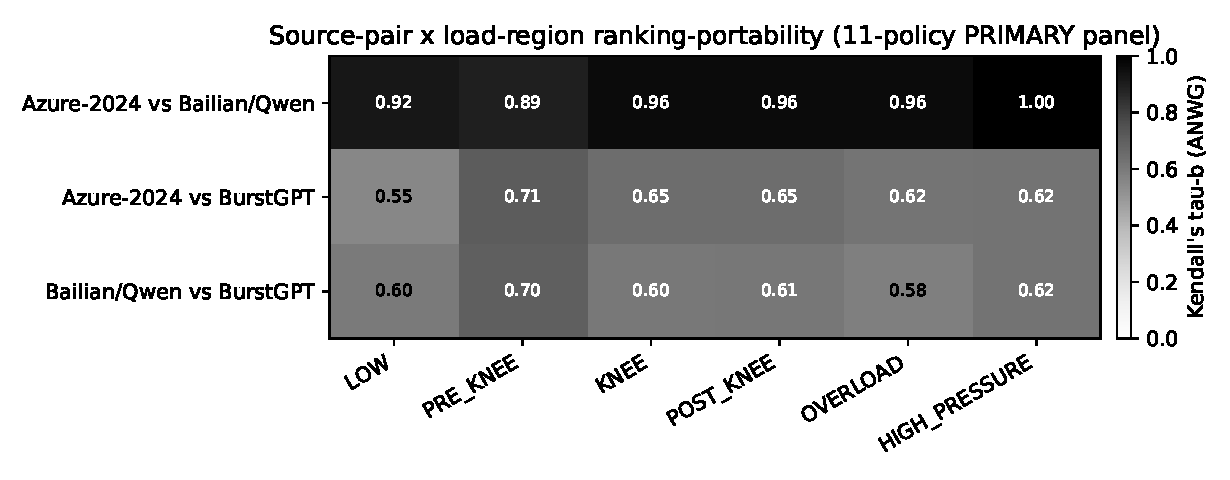
\includegraphics[width=0.85\textwidth]{generated/figures/fig1_portability_heatmap.pdf}
\caption{Source-pair $\times$ load-region ranking-portability: Kendall's
tau-b between each pair of sources' PRIMARY-panel (11-policy) rankings on
the ANWG metric, at each of the six frozen operating regions
(\S\ref{sec:calibration}). Computed from the frozen ranking correlations artifact.}
\label{fig:portability-heatmap}
\end{figure}

The min/max range in Table~\ref{tab:rq1-by-region} makes clear that
portability is not homogeneous even within a region: the range at LOW
($0.55$--$0.92$) is nearly as wide as at any other region, and the range is
driven entirely by which source pair is compared, not by which region is
compared (\S\ref{sec:load-conditioning} tests region dependence
explicitly). No region shows uniformly low or uniformly high agreement
across all three source pairs simultaneously.

\subsection{Load Conditioning}
\label{sec:load-conditioning}

Load-level dependence is a secondary robustness/sensitivity analysis
(\S\ref{sec:rq}), reported here as a direct read of the same
\S\ref{sec:cross-source-rankings} table rather than a separate headline
claim of cross-source rank instability by itself. Secondary ranking statistics (Spearman's $\rho$ and top-1/top-3 overlap) exhibit an identical quantitative pattern and are omitted from the main tables for concision; their full values are preserved in the released analysis outputs. Table~\ref{tab:rq1-by-region}'s
per-region mean tau-b is close to flat across the six regions ($0.69$ at
LOW, rising to $0.72$--$0.77$ elsewhere, no monotonic trend with load
factor); a leave-one-region-out comparison between the full six-region
grid and the four-region \texttt{LOW}/\texttt{PRE\_KNEE}/\texttt{KNEE}/
\texttt{OVERLOAD} subset used by \texttt{LOAD\_CALIBRATION\_SENSITIVITY}
(\S\ref{sec:robustness}) changes the mean tau-b by less than $0.01$
($0.728$ on the four-region subset versus $0.733$ on the full six-region
grid) -- the headline cross-source portability conclusion is not sensitive
to the choice of four-region versus six-region calibration grid. Load
regime does, however, materially affect \emph{where practically supported
reversals occur} (\S\ref{sec:reversals}): reversal counts are concentrated
at PRE\_KNEE and above, essentially absent at LOW.

\subsection{Pairwise Reversals}
\label{sec:reversals}

Of the 990 (policy pair) $\times$ (source pair, region) PRIMARY-metric
records (55 policy pairs among the 11 PRIMARY policies $\times$ 18
conditions), the
five-class breakdown (\S\ref{sec:uncertainty}) is: $906$
\texttt{STABLE\_NO\_SIGN\_CHANGE} ($91.5\%$), $48$
\texttt{MICROSCOPIC\_SIGN\_CHANGE} ($4.8\%$), $36$
\texttt{SUPPORTED\_PRACTICAL\_REVERSAL} ($3.6\%$), and zero records in
either \texttt{UNDEFINED\_UNESTIMABLE} or
\texttt{UNSUPPORTED\_SIGN\_CHANGE\_WIDE\_CI}. The large majority of
pairwise comparisons are stable; a small but non-trivial minority (about 1
in 28) are both practically and statistically supported reversals -- never
a majority, and never absent. That zero records fall into
\texttt{UNSUPPORTED\_SIGN\_CHANGE\_WIDE\_CI} means that, at this sample
size, every sign change with a practically meaningful margin also had a
statistically supported direction, and vice versa -- on this data the
practical-margin and statistical-support criteria never disagreed with each
other; this is a description of the observed record set, not independent
confirmation that the two criteria would always agree.

\begin{figure}[h]
\centering
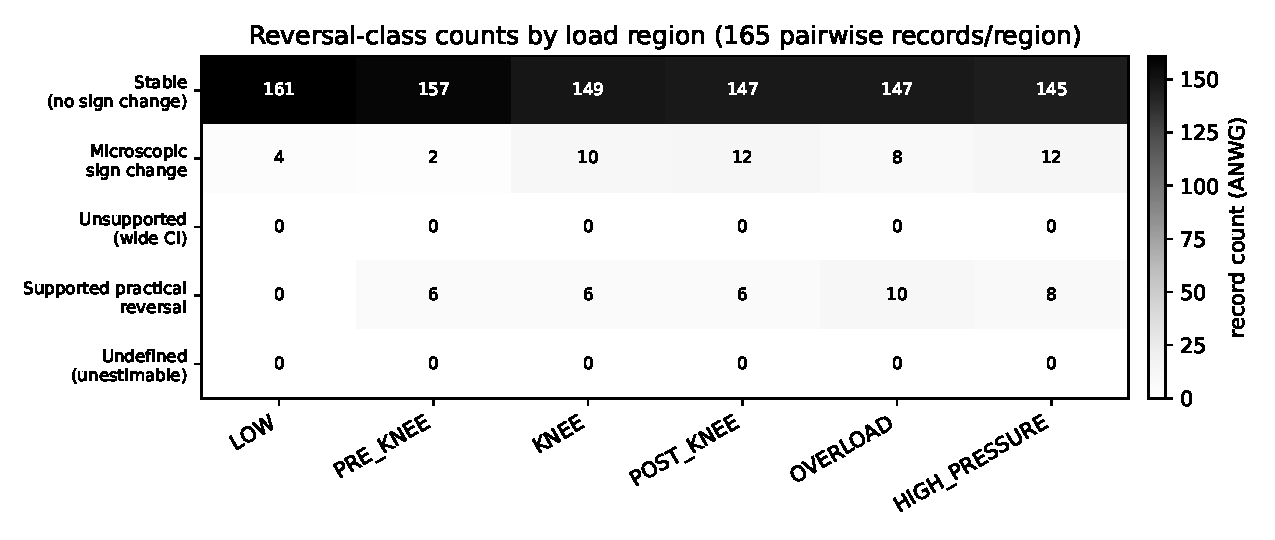
\includegraphics[width=0.85\textwidth]{generated/figures/fig2_reversal_class_matrix.pdf}
\caption{Reversal-class counts by operating region, PRIMARY metric (165
pairwise records per region: 55 policy pairs $\times$ 3 source pairs).
Computed from the frozen pairwise reversals artifact.}
\label{fig:reversal-matrix}
\end{figure}

Reversal counts are load-dependent: zero \texttt{SUPPORTED\_PRACTICAL\_REVERSAL}
records at \texttt{LOW}, rising to 6 at each of \texttt{PRE\_KNEE},
\texttt{KNEE}, and \texttt{POST\_KNEE}, 10 at \texttt{OVERLOAD}, and 8 at
\texttt{HIGH\_PRESSURE} (Figure~\ref{fig:reversal-matrix}). Every one of
the 36 PRIMARY-metric supported reversals that we manually inspected in
the underlying record set involves the same two policies,
\texttt{slai\_faithful} and \texttt{vllm\_faithful}, and every one is a
\emph{cross-source} reversal in which one side of the comparison is a
BurstGPT condition -- consistent with \S\ref{sec:cross-source-rankings}'s
finding that BurstGPT is the source pair member most associated with lower
agreement. The single largest-effect-size supported reversal (operationalized
as the smaller-magnitude of the two conditions' practical margins, the
binding constraint under the frozen practical-margin rule,
\S\ref{sec:uncertainty}) is \texttt{slai\_faithful} vs.\
\texttt{vllm\_faithful} at \texttt{HIGH\_PRESSURE}, comparing Azure-2024
(or, at an effectively tied effect size, Bailian/Qwen) against BurstGPT --
this is the case selected for real-system validation under the frozen
selection rule (\S\ref{sec:real-system}).

A representative stable comparison, used as a null-result control alongside
the reversal case in the real-system validation design
(\S\ref{sec:real-system}), is the source pair with both the highest tau-b
and (among the highest-tau conditions) the narrowest bootstrap interval:
Azure-2024 vs.\ Bailian/Qwen at \texttt{HIGH\_PRESSURE} ($\tau = 1.00$,
95\% CI $[0.90, 1.00]$).

\subsection{Temporal Portability}
\label{sec:temporal}

Following the frozen temporal design (\S\ref{sec:temporal-design}), four
temporal record types are reported separately, each under its source's own
chronology, and never merged into a single ``temporal/domain OOD'' number:
BurstGPT's EARLY/MIDDLE/LATE tercile split (primary) and EARLY/LATE bisect
(sensitivity check on the tercile boundary), Azure-2024's absolute calendar
split, and Bailian/Qwen's \texttt{RELATIVE\_CHRONOLOGY\_ONLY} comparison,
for which no calendar-based claim is made. All values are keyed identically
to the source temporal robustness artifact. The canonical results reveal high rank stability across time: BurstGPT's tercile split shows strong agreement between EARLY and LATE chunks across non-LOW load regions ($\tau_b \in [0.81, 1.0]$), while the BISECT sensitivity check yields similarly stable correlations ($\tau_b \in [0.72, 0.80]$). Azure's calendar split produces near-perfect correlation ($\tau_b \in [0.90, 1.0]$), and Bailian's relative-chronology split likewise exhibits minimal rank change ($\tau_b \in [0.94, 1.0]$).

Although the frozen protocol for this research question specified an analysis of temporal, provider, and domain shifts, a standalone domain-shift component was not separately operationalized in the final artifacts. The evidence reported here addresses the temporal component directly. The frozen cross-source comparisons (\S\ref{sec:cross-source-rankings}) include the one genuine provider boundary in this corpus (Bailian/Qwen on Alibaba Cloud versus the two Microsoft-infrastructure sources, \S\ref{sec:sources}), but the design does not isolate a causal provider effect from ordinary cross-source variation -- BurstGPT-vs-Azure is a cross-source, not cross-provider, comparison; domain shift, like the provider component, is addressed only implicitly through these same cross-source comparisons and was not separately operationalized.

\subsection{Robustness}
\label{sec:results-robustness}

Of the seven preregistered robustness families (\S\ref{sec:robustness}), six were computed (five in the ranking-correlation, temporal-robustness, and sample-complexity outputs below, and a sixth, \texttt{LEAVE\_ONE\_POLICY\_FAMILY\_OUT}, in the telemetry-explanation analysis of \S\ref{sec:telemetry-explanation}). The seventh, \texttt{METRIC\_DEFINITION\_SENSITIVITY}, was never implemented; we disclose this as a protocol gap rather than perform a post hoc analysis after the results were already known.

\begin{itemize}
  \item \textbf{\texttt{PRIMARY\_ONLY}.} Identical to the headline result
    by construction: the ranking correlations artifact already restricts
    every comparison to the 11-policy PRIMARY panel
    (\S\ref{sec:cross-source-rankings}), never mixing in the two
    \texttt{STYLE\_APPROXIMATION} robustness policies.
  \item \textbf{\texttt{LEAVE\_ONE\_SOURCE\_OUT}.} Excluding BurstGPT
    leaves only the Azure-2024/Bailian-Qwen pair, whose mean tau-b is
    $0.948$ -- close to the ceiling. Excluding Azure-2024 or Bailian/Qwen
    each leaves a BurstGPT-involving pair, with mean tau-b $0.633$ and
    $0.618$ respectively. This is the same asymmetry as
    \S\ref{sec:cross-source-rankings}, now stated per excluded source: the
    headline portability figure is high specifically because two of the
    three sources agree strongly, and is pulled down specifically by
    BurstGPT, not uniformly by all three sources.
  \item \textbf{\texttt{LOAD\_CALIBRATION\_SENSITIVITY}.} Reported in
    \S\ref{sec:load-conditioning}: mean tau-b changes by less than $0.01$
    between the four- and six-region grids.
  \item \textbf{\texttt{TEMPORAL\_SPLIT\_SENSITIVITY}.} The BurstGPT
    bisect-vs-tercile comparison from \S\ref{sec:temporal}; both split
    definitions are reported side by side in the released table rather
    than collapsed into one number.
  \item \textbf{\texttt{WINDOW\_SIZE\_SENSITIVITY}.} Despite its name,
    this item is the window-\emph{count} subsampling ladder of
    \S\ref{sec:sample-complexity}, not a requests-per-window sweep
    (\S\ref{sec:window-size}), and is not separately recomputed here.
  \item \textbf{\texttt{LEAVE\_ONE\_POLICY\_FAMILY\_OUT}.} Excluding any
    single one of the ten frozen mechanism families changes the headline
    mean tau-b only modestly, from $0.707$ (excluding the classical
    arrival-order family) to $0.792$ (excluding the SLO-aware family),
    against the full-panel baseline of $0.733$. No single mechanism
    family's removal collapses or inflates the headline portability
    figure -- the source-pair-driven pattern of
    \S\ref{sec:cross-source-rankings} is not an artifact of any one
    policy family dominating the panel.
\end{itemize}

\subsection{Cross-Metric Ranking Portability}
\label{sec:results-cross-metric}

\S\ref{sec:reversals} and \S\ref{sec:results-robustness} ask whether a
policy ranking under one fixed metric (ANWG) is portable across sources,
regions, and windows. A different question -- whether a ranking is
portable across \emph{metrics}, for the same source and region -- is
addressed here as an explicitly labeled post-campaign extension that
reuses the primary analysis's own statistical methods without modifying,
re-running, or re-deriving the underlying outcome matrix. Across all $3$
sources $\times$ $6$ regions $\times$ $55$
metric pairs among the study's tracked outcome metrics ($990$ conditions),
rank correlation between metrics is on average moderate (median Kendall's
$\tau_b = 0.419$, range $[-0.506, 1.000]$; $202/990$, $20\%$, of conditions
have \emph{negative} $\tau_b$), and the single top-ranked policy agrees
between the two metrics in only $316/990$ ($31.9\%$) of conditions
(disagreeing in the remaining $68.1\%$). At the level of individual
pairwise policy comparisons ($54{,}450$ total, one per (metric pair, condition, policy pair), generated from the 55 unique pairs among the 11 eligible tracked metrics: ANWG, completion fraction, weighted completion fraction, SLO-violation rate, weighted goodput, mean latency, p95 latency, request throughput, token throughput, mean TTFT, and p95 TTFT; p99 latency was ineligible and excluded), the same five-class taxonomy as \S\ref{sec:reversals} (ordinary, not
FDR-adjusted, bootstrap-CI classification; \S\ref{sec:uncertainty}) finds $3{,}244$ ($6.0\%$) show a statistically
supported practical disagreement in which
policy is preferred depending on which metric is used, versus $45{,}800$
($84.1\%$) in the same order, $5{,}205$ ($9.6\%$) a sign change too small
to be practically meaningful, and $201$ ($0.4\%$) an unsupported sign
change with a wide confidence interval; no comparison in this policy panel
was undefined or unestimable. Unlike \S\ref{sec:reversals}'s primary
reversal check, the separate BH-FDR correction removes some of these
cross-metric disagreements: of the $3{,}244$ raw-CI-supported records,
$3{,}207$ ($98.9\%$) also survive the family-wise BH-FDR check, while
$37$ ($1.1\%$) do not, meaning the multiplicity-corrected count of
cross-metric disagreements is $3{,}207$ rather than $3{,}244$ -- a genuine,
disclosed sensitivity to the multiplicity correction, not an error in
either figure. Scheduler-ranking portability is
therefore not only source- and region-dependent (\S\ref{sec:results});
which metric is used to define ``better'' materially changes the ranking
in a non-trivial minority of conditions, and the median condition shows no
default expectation that the two metrics' top choices should agree.

\subsection{SLO-Definition Sensitivity}
\label{sec:results-slo}

As disclosed in \S\ref{sec:slo-sensitivity-gap}, this check was never part
of the preregistered protocol; we report it here as the post-campaign
extension it was actually run as: three alternative SLO-synthesis
multipliers (\texttt{tight\_10x}, \texttt{primary\_20x} -- this study's own
convention -- and \texttt{loose\_40x}) applied across the 5 load regions
that contain at least one PRIMARY-metric supported reversal (excluding
\texttt{LOW}, which accounts for 0 of the 36 supported reversals and so
has nothing for a sensitivity check to stress-test), evaluating $11$
policies $\times$ $120$ total windows $\times$ $5$ regions $\times$ $3$
variants ($19{,}800$ cells; 0 failed), with every seed held identical to
\S\ref{sec:results}.

\textbf{Ranking robustness.} Across the $30$ (source, region, variant)
conditions compared against the study's primary SLO convention, rank
correlation stays high under either alternative (median Kendall's
$\tau_b = 0.872$, range $[0.533, 1.000]$); the single top-ranked policy
nonetheless changes under an alternative SLO definition in $13/30$ ($43\%$)
of conditions.

\textbf{Reversal persistence.} We check the 36 PRIMARY-metric supported reversals from \S\ref{sec:reversals} against the alternative definitions. Because there are 3 SLO variants (tight, primary, loose), there are $36 \times 3 = 108$ mathematical comparisons in the artifact's persistence matrix, of which $36$ are identity checks against the primary definition itself (all 36 trivially persist). Restricting focus to the $72$ scientifically meaningful non-trivial comparisons against the alternative definitions: $52/72$ ($72\%$) persist, $6/72$ ($8\%$) change direction, $10/72$ ($14\%$) remain the same direction but fall below the practical-margin threshold under the alternative definition, and $4/72$ ($6\%$) become statistically indistinguishable from zero. No headline reversal from \S\ref{sec:reversals} is contradicted outright, but a non-trivial minority ($20/72$, $28\%$) are sensitive to the SLO-definition
choice -- disclosed here as a caveat on those specific reversals, not
grounds to discard them.

\subsection{Synthetic-to-Real Ranking Transfer (Pilot, Not Headline Evidence)}
\label{sec:results-rq3-pilot}

RQ3 (\S\ref{sec:study-design}) is preregistered as a SECONDARY question,
never a headline result contract item. We report only an engineering-
validation pilot of the synthetic-to-real transfer pipeline: $176/176$
pilot cells executed and $24/24$ analysis records generated, $0$ schema-validation
or telemetry failures, across all $4$ synthetic stress families
(\texttt{burst\_arrival}, \texttt{decode\_length\_skew},
\texttt{heavy\_tail\_service}, \texttt{priority\_slo\_heterogeneity}), both
selected load regions, and all $3$ real sources. By design, the pilot uses
only $2$ synthesis seeds per family, too few for the frozen block-bootstrap
transfer statistic to be defined in most conditions: Kendall's $\tau_b$ is
undefined (\texttt{null}, insufficient sign pairs) in $21/24$ ($88\%$)
pilot conditions. \textbf{We therefore draw no synthetic-to-real transfer
conclusion, positive or negative, from this pilot}; it establishes only
that the pipeline executes correctly end-to-end. A full-scale extension
(targeted, not exhaustive) with sufficient seeds per family to define the
transfer statistic is left to future work, consistent with RQ3's
SECONDARY, non-headline status in this study's frozen contract.

\section{Benchmark Sample Complexity}
\label{sec:sample-complexity}

\subsection{Motivation}
\label{sec:sample-complexity-motivation}

Every scheduler-ranking result in this manuscript is itself derived from a
finite window budget -- 40 windows per source, 120 total
(\S\ref{sec:windows}). A systems researcher designing a future scheduler
comparison faces a practical, resource-bound version of the same question
this benchmark studies at the source/region/metric level: \emph{if only $n$
workload windows can be afforded, how reliably would the resulting
scheduler-ordering conclusion reproduce the conclusion obtained from the
full window collection?} This question is itself a systems-evaluation
parameter, not a purely statistical afterthought: it bounds the
experimental cost of a trustworthy scheduler comparison, it affects how
much confidence a reader should place in a paper that evaluates on a
handful of trace windows, and it is a precondition for treating this
benchmark's own frozen 120-window corpus (rather than some larger or
smaller corpus) as an adequate evidentiary base for the results in
\S\ref{sec:results}.

\subsection{Design}
\label{sec:sample-complexity-design}

For the PRIMARY metric, recovery of the exact $n=40$ reference ranking is
slow and strongly source-dependent (Figure~\ref{fig:sample-complexity},
Table~\ref{tab:rq4-first-n}): BurstGPT never reaches the preregistered
$0.9$ exact-order recovery threshold below the full window budget ($0.2\%$
at $n=5$, rising only to $56.6\%$ at $n=30$), Bailian/Qwen similarly does
not cross $0.9$ before $n=40$ ($64.0\%$ at $n=30$), while Azure-2024
crosses the threshold already at $n=30$ ($98.8\%$). None of the three
sources reaches $0.9$ exact-order recovery at $n \in \{5,10,20\}$. Because
$n=40$ is the size of the full reference pool itself, exact recovery at
$n=40$ is $1.0$ by construction (sampling all 40 windows without
replacement reproduces the reference exactly) and is not an informative
data point on its own; the informative content is in how slowly each
source's curve rises toward that trivial ceiling.

Top-1 recovery (does the resampled subset identify the single
best-performing PRIMARY-panel policy correctly) is a materially easier
question than exact-order recovery for two of the three sources: Azure-2024
and Bailian/Qwen both exceed $0.9$ top-1 recovery already at $n=5$
($96.6\%$ and essentially $100\%$ respectively), even though their
\emph{exact}-order recovery at $n=5$ is only $35.0\%$ and $14.6\%$. For
these two sources, identifying the single best policy requires far less
evidence than reconstructing the complete 11-policy ordering. BurstGPT
shows no such gap: its top-1 recovery is comparably slow to its
exact-order recovery ($13.0\%$ at $n=5$, $74.2\%$ at $n=30$, not reaching
$0.9$ within the tested ladder either) -- consistent with
\S\ref{sec:cross-source-rankings}'s finding that BurstGPT is the source
whose relative ordering is hardest to pin down. Comparing a concentrated
(single-source-heavy) against a distributed (evenly-spread-across-sources)
window budget of equal total size, the distributed budget achieves higher
mean Kendall's tau-b against the reference ranking ($0.986$) than the
concentrated budget ($0.940$) for the primary metric -- spreading a fixed
evaluation budget across sources recovers the reference ranking more
reliably than concentrating it in one source.

\begin{table}[h]
\centering
\caption{Smallest $n$ at which PRIMARY-metric recovery probability first
exceeds $0.9$ (blank = not reached within the tested ladder,
$n \in \{5,10,20,30,40\}$).}
\label{tab:rq4-first-n}
\begin{tabular}{lcc}
\toprule
Source & first $n$, exact-order $\geq 0.9$ & first $n$, top-1 $\geq 0.9$ \\
\midrule
Azure-2024    & 30 & 5 \\
Bailian/Qwen  & 40 & 5 \\
BurstGPT      & 40 (not reached below 40) & not reached \\
\bottomrule
\end{tabular}
\end{table}

\begin{figure}[h]
\centering
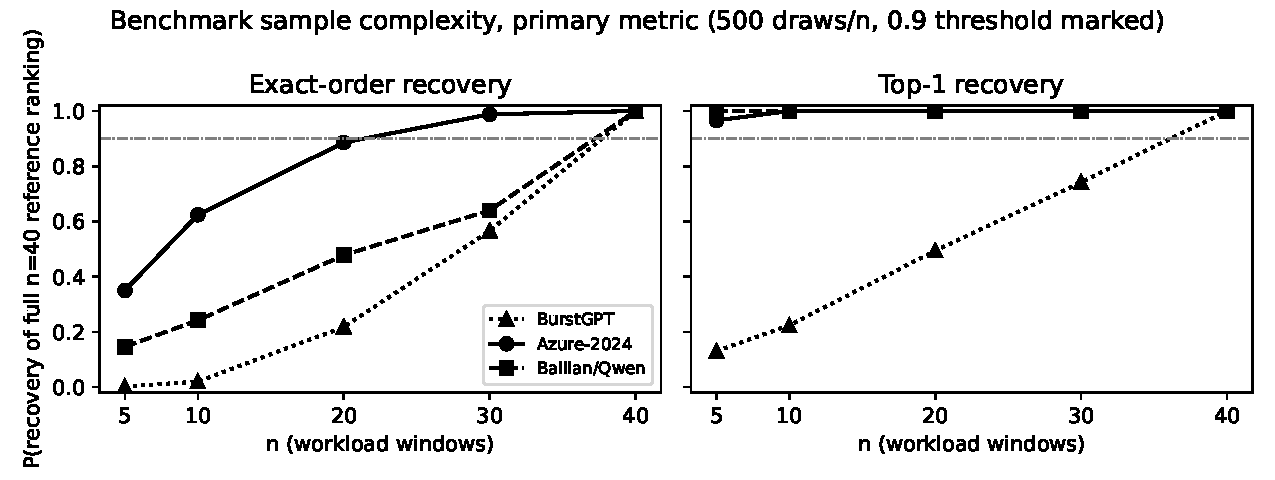
\includegraphics[width=\textwidth]{generated/figures/fig3_sample_complexity_curves.pdf}
\caption{Benchmark sample-complexity recovery curves, PRIMARY metric, 500
draws per $n$, sampling without replacement. Left: exact-order recovery of
the full $n=40$ reference ranking. Right: top-1 recovery. The $0.9$
threshold is marked. Computed from \texttt{sample\_complexity.json}
(SHA-256 \texttt{cb54afc0\ldots}).}
\label{fig:sample-complexity}
\end{figure}

This analysis directly answers RQ5 (\S\ref{sec:rq}) and depends on the full
Pilot-V2 outcome matrix (\S\ref{sec:results}); it is not run on Stage-0's
historical, smaller pilot (\S\ref{sec:stage0}).

\section{Real-System Model-Fidelity Validation}
\label{sec:real-system}

\subsection{Objective}
\label{sec:real-system-objective}

This analysis addresses RQ6 (\S\ref{sec:rq}) as a selected
model-fidelity and domain-of-validity check. We do not claim that simulated
absolute latency or throughput values match real-hardware values; simulator
latency is not assumed to transfer directly to real-engine latency, nor is
the simulator's own load-calibration reference $\lambda_{\mathrm{ref}}$
(\S\ref{sec:calibration}) expected to transfer to a physical engine's
saturation point. The sole objective of this validation is to test agreement
in \emph{relative policy ordering} and \emph{reversal direction} between
the simulator and a real vLLM deployment on a targeted set of validation
cases. Agreement would support the selected simulated comparison; a
disagreement would instead identify a boundary on how that simulated
comparison should be interpreted.

\subsection{Experimental Design}
\label{sec:real-system-design}

The real-system validation follows a preregistered, window-resampled
evaluation design structured to mirror the simulated campaign without
requiring exhaustive duplication. It is deliberately not a full physical
re-execution of the 13-policy, six-region simulation matrix. The evaluation
protocol is defined as follows:

\begin{itemize}
  \item \textbf{Inferential Unit:} The statistical unit of analysis is the workload window, preserving the methodology established in \S\ref{sec:methodology}.
  \item \textbf{Scale and Execution:} The design evaluates $40$ independent workload windows per source, each containing $200$ requests. Exactly one scientific execution is performed per (policy, source, window) cell, yielding $240$ total scientific tasks ($2$ policies $\times$ $3$ sources $\times$ $40$ windows).
  \item \textbf{Uncertainty Quantification:} Uncertainty is quantified via window-level bootstrap resampling ($\ge 2{,}000$ resamples) over the $40$ independent windows per source.
  \item \textbf{Operating Regions:} Workloads are calibrated against the real engine's observed saturation point to define load regions independently of the simulator's calibration.
  \item \textbf{Software and Hardware:} Every execution serves \texttt{Qwen/Qwen2.5-0.5B-Instruct} on \texttt{vllm==0.27.1} (\texttt{torch==2.13.0}), one instance per task on a single NVIDIA A100-SXM4-80GB GPU (Slurm resource label \texttt{gres=gpu:a100\_10g}, unchanged from the validated load-calibration campaign). This label is a Slurm resource tag, not evidence of a fractional or MIG GPU partition; the allocated device is a full 80\,GB A100. Tokenizer revision, model dtype, tensor-parallel degree, and maximum model length were not separately recorded in the frozen execution manifest; rather than invent values, we do not report them here.
  \item \textbf{Ordering and Provenance:} Each (policy, source, window) cell is executed exactly once; with one execution per cell there is no repeated-measures ordering to alternate. Cells are assigned deterministically to Slurm array indices by a fixed (source, window, policy) sort, with execution concurrency limited to four simultaneous array tasks. Every execution records its exact git commit, hardware environment (per-task GPU query), software versions, and workload/calibration-manifest hash identity to ensure reproducibility.
\end{itemize}

\subsection{Case Selection}
\label{sec:real-system-case-selection}

Validation cases were selected mechanically from the validated results presented in \S\ref{sec:reversals}, applying a preregistered rule that prefers the pairwise reversal with the largest effect size and a representative stable-ordering control.

\begin{itemize}
  \item \textbf{Reversal Case:} \texttt{slai\_faithful} versus \texttt{vllm\_faithful}, comparing the Azure and BurstGPT sources at high load. This case exhibited the largest-effect-size statistically supported practical reversal in simulation (a simulator difference of $+0.520$ for Azure favoring \texttt{slai\_faithful}, and $-0.348$ for BurstGPT favoring \texttt{vllm\_faithful}).
  \item \textbf{Stable Control:} Azure versus Bailian/Qwen at high load, chosen for exhibiting perfect rank agreement in simulation.
\end{itemize}

Evaluating this selection on physical hardware requires mapping the simulated mechanisms to their real-engine equivalents. While \texttt{vllm\_faithful} maps directly to native vLLM execution paths, the SLO-aware SLAI/RAD mechanism requires a custom vLLM scheduling plugin to realize its semantics on real hardware.

\subsection{Results}
\label{sec:real-system-result}

The physical-hardware load-calibration prerequisite for these validation cases has been executed (120/120 terminal outcomes: 43 converged, 77 lower-bound-already-violating), establishing the necessary injection rates for the deployment environment. All $240$ scientific evaluation tasks ($2$ policies $\times$ $3$ sources $\times$ $40$ windows) subsequently completed on the software/hardware environment above (\S\ref{sec:real-system-design}), with zero failed, timed-out, or partial cells.

Table~\ref{tab:rq6-results} reports the \texttt{slai\_faithful}-minus-\texttt{vllm\_faithful} arrival-normalized-weighted-goodput (ANWG) effect for each source, using the same window-level paired bootstrap as \S\ref{sec:uncertainty} ($2{,}000$ resamples over the $40$ independent windows/source, 95\% CI). All three effects are statistically supported (CI excludes zero) and favor \texttt{vllm\_faithful}.

\begin{table}[t]
\centering
\caption{Real-vLLM RQ6 outcomes against the simulator-selected cases (\texttt{HIGH\_PRESSURE}, 40 paired windows/source, 95\% window-level bootstrap CI, $2{,}000$ resamples). Effect is \texttt{slai\_faithful}$-$\texttt{vllm\_faithful} ANWG.}
\label{tab:rq6-results}
\small
\setlength{\tabcolsep}{4.5pt}
\resizebox{\textwidth}{!}{%
\begin{tabular}{lccccl}
\toprule
Source & Sim.\ winner & Effect & 95\% CI & Real winner & Agreement \\
\midrule
Azure (rev.) & SLAI ($+0.520$) & $-0.024$ & $[-0.027,-0.020]$ & vLLM & Disagrees \\
BurstGPT (rev.) & vLLM ($-0.348$) & $-0.200$ & $[-0.264,-0.144]$ & vLLM & Agrees \\
Bailian (ctrl.) & n/a$^{*}$ & $-0.026$ & $[-0.030,-0.022]$ & vLLM & Consistent \\
\bottomrule
\end{tabular}
}
\vspace{2pt}

{\footnotesize $^{*}$The simulator's stable-control quantity ($\tau_b = 1.00$) is an
11-policy full-ranking correlation, not a two-policy \texttt{slai\_faithful}-vs-\texttt{vllm\_faithful}
winner; no directly comparable simulator winner is defined for this row. The
relevant real-system check is instead whether the two-policy ordering agrees
between the Azure and Bailian/Qwen conditions, which it does (both favor
\texttt{vllm\_faithful}).}
\end{table}

The simulator-predicted Azure/BurstGPT reversal did not reproduce:
\texttt{vllm\_faithful} won both conditions on real hardware, so the
predicted sign flip between Azure and BurstGPT was not observed. BurstGPT's
real winner matches the simulator's selection; Azure's does not -- the
physical Azure comparison changed from a simulated \texttt{slai\_faithful}
advantage to a small but statistically supported \texttt{vllm\_faithful}
advantage. This negative validation result is scientifically informative:
it identifies a fidelity boundary for the selected simulator-predicted
major reversal and prevents that simulated reversal from being read as a
hardware-confirmed result. In contrast, the Azure/Bailian-Qwen
stable-control comparison retained a consistent \texttt{vllm\_faithful}-
favoring ordering across both real-system conditions (effect magnitudes
$-0.0235$ and $-0.0256$), reproducing the qualitative stability that
comparison was selected to test, independent of which specific policy wins.

Statistical support is not the same as practical magnitude. Read against
this study's 10\% practical-margin convention (\S\ref{sec:uncertainty}),
the three real-system effects vary substantially once expressed relative
to the losing policy's own mean ANWG (frozen descriptive aggregates,
\texttt{docs/RQ6\_PUBLIC\_RESULT\_PROVENANCE.md}): Azure's margin is
$(0.7700-0.7465)/0.7465 \approx 3.1\%$ and Bailian/Qwen's is
$(0.84525-0.819625)/0.819625 \approx 3.1\%$ -- both statistically
supported but below the 10\% convention used elsewhere in this study to
separate practically meaningful from microscopic effects. BurstGPT's
margin, $(0.316625-0.116375)/0.116375 \approx 172\%$, substantially
exceeds it. This is a descriptive comparison against an existing
convention, not a new inferential analysis: \S\ref{sec:uncertainty}'s
five-class taxonomy is defined for a pairwise comparison across two
conditions of the same source and is not applied here to a single
physical-source row.

This selected-case result exposes a simulator-fidelity boundary rather
than establishing a general finding: the Azure/BurstGPT reversal that the
simulator identified as this study's largest-effect-size case did not
transfer to physical execution, while the paired stable-control comparison
retained its qualitative ordering (\S\ref{sec:threats} scopes what this
design does and does not establish; \S\ref{sec:discussion} interprets the
two outcomes together). The appropriate interpretation is therefore not
that simulation should be discarded, but that simulation-derived
comparative rankings require an explicit model-validity context.

\section{Discussion}
\label{sec:discussion}

The result (\S\ref{sec:results}) is neither cleanly ``portable'' nor
cleanly ``fragile'' -- it is source-pair-dependent in a specific,
mechanistically legible way, and that dependence itself is the finding.

\subsection{Portability Is Real but Source-Pair-Dependent, Not Uniform}

Comparative scheduler rankings are never uncorrelated between any two
sources at any region (\S\ref{sec:cross-source-rankings}): a scheduler
comparison performed on one of this study's three sources is never
scientifically meaningless evidence about the others. At the same time,
portability is far from uniform, and the non-uniformity is legible rather
than diffuse: Azure-2024 and Bailian/Qwen agree almost perfectly at every
operating region, while every comparison involving BurstGPT is consistently
lower (\S\ref{sec:cross-source-rankings},
\S\ref{sec:results-robustness}). The
practical implication is neither ``a small, well-chosen evaluation
footprint always suffices'' nor ``every scheduler comparison must be
re-verified on every workload'': it is that \emph{which} second source a
comparison is checked against matters more than \emph{whether} a second
source is checked at all. A comparison validated only on Azure-2024-like
traffic transfers with high confidence to Bailian/Qwen-like traffic under
this study's panel and metric, but the same transfer to BurstGPT-like
traffic is measurably less reliable, and that reliability gap holds at
every load level tested, not only under stress.

\subsection{Practically Supported Reversals Are Real, Uncommon, and
Load-Concentrated}

Practically and statistically supported reversals are a small minority of
PRIMARY-metric pairwise comparisons (\S\ref{sec:reversals}), but not zero,
and not dismissible as measurement noise: the same bootstrap procedure
classifies the large majority of comparisons as stable. Every supported
reversal we examined is the same policy pair and involves BurstGPT on one
side, and reversals are not spread evenly across the operating envelope;
they concentrate at and above \texttt{PRE\_KNEE}. A scheduler comparison performed only at low load,
even on a source pair that is otherwise highly portable, would have missed
every reversal this benchmark found. This motivates evaluating scheduler
comparisons across an operating curve, not at a single convenient load
point, as this benchmark's design already does
(\S\ref{sec:calibration}).

\subsection{Practical Implications for Benchmark Design}

Two implications follow directly and are not deployment recommendations
about which scheduler to use, only about how to evaluate schedulers
credibly. First, a comparison checked against only one additional workload
source cannot be assumed representative of ``other workloads'' in
general -- which specific source is used as the check matters, and
BurstGPT-like traffic in particular is where this study's evidence
concentrates its cross-source disagreement. Second, benchmark sample
complexity is itself load- and metric-behavior-relevant evidence:
\S\ref{sec:sample-complexity}'s finding that exact-order recovery requires
the full window budget for two of three sources, while top-1 recovery is
achievable from very few windows for those same two sources, means a
researcher who only needs to know ``which scheduler is best'' faces a
different, much smaller evidence requirement than one who needs the
complete ordering -- a distinction a single point-estimate benchmark
result cannot convey on its own.

\subsection{Portability Also Depends on Which Metric and Which SLO
Definition Is Used}

\S\ref{sec:cross-source-rankings}--\S\ref{sec:reversals} establish that a
ranking's portability depends on which \emph{workload source} it is checked
against. \S\ref{sec:results-cross-metric} and \S\ref{sec:results-slo} show
that portability depends, independently, on which \emph{metric} and which
\emph{SLO definition} is used to compute the ranking in the first place --
two further conditioning variables, not a repetition of the source-pair
finding above.

The cross-metric result is the more consequential of the two. Rank
correspondence across metric pairs is only moderate (median
$\tau_b = 0.419$) -- well below the agreement between the two most portable
\emph{sources} -- and metrics sometimes rank policies in opposite order
rather than merely disagreeing in degree. For a randomly chosen (source,
region) condition, which metric is used changes which policy comes out on
top more often than not (\S\ref{sec:results-cross-metric}).
This does not mean
metrics are arbitrary or that any one choice is as good as another -- ANWG,
completion fraction, and the latency- and SLO-based metrics measure
genuinely different deployment objectives (\S\ref{sec:metrics}), and a
practitioner optimizing for tail latency has no reason to expect the same
ranking as one optimizing for weighted goodput. The finding is instead that
\emph{which} objective a benchmark reports on is as much a part of the
ranking-portability question as which workload it was measured on, and a
scheduler comparison that reports only its primary metric is silent on
whether that comparison would hold under a deployment's actual objective.

The SLO-definition result is distinct from metric sensitivity and
comparatively reassuring, but not a clean pass: ranking robustness under
alternative SLO-synthesis conventions is closer to the cross-source ceiling
than to the cross-metric result, yet the top-ranked policy and a non-trivial
minority of specific reversals do change with the SLO definition
(\S\ref{sec:results-slo}). The practical reading is narrower than either
``robust'' or ``fragile'': a scheduler conclusion can remain broadly
ordered under a nearby SLO definition even while its winning policy, or a
specific reversal a reader cares about, does not.

Taken together with \S\ref{sec:cross-source-rankings}'s source-pair finding
and \S\ref{sec:reversals}'s load-concentration finding, this study's central
conclusion is that a comparative scheduler claim is conditional on at least
four axes -- workload source, operating region, evaluation metric, and (for
deadline-dependent policies) SLO definition -- and reporting a ranking
without stating which values of each axis produced it risks the ranking
being read as more general than the evidence supports.

\subsection{Explanatory Telemetry: A Preliminary, Heavily Qualified Read}
\label{sec:telemetry-explanation}

The frozen, pre-specified explanatory model (\S\ref{sec:telemetry})
associates the five workload
descriptors with reversal sites at each (policy pair, condition) cell, but
converges with a usable sample size ($\geq 20$ observations) for only 42 of
990 cells -- most reversal sites are too sparse for this per-cell model to
fit reliably, and the frozen output records point coefficients only, with
no standard errors or significance test. Any reading of this evidence must
therefore be provisional. Within that small, non-significance-tested set,
\texttt{prompt\_tokens\_cv} has a negative coefficient in 39 of 42 cells --
the most consistent single direction among the five descriptors -- which
is at least \emph{consistent with} (not confirmatory of) prompt-length
variability being associated with where reversals occur, echoing
\S\ref{sec:drivers}'s finding that prompt-length structure is the
classifier's most predictive, non-redundant feature for source
separability itself. The other four descriptors show
weaker, closer-to-even sign splits across the interpretable cells and do
not support a directional claim. We do not read this as evidence that any
descriptor \emph{causes} a reversal: because the sources are themselves
observably separable (\S\ref{sec:separability}), an association between a
descriptor and a reversal may reflect only a source-separating feature that
co-occurs with where reversals were or were not observed. It is a candidate
association worth a properly powered, purpose-built follow-up study;
consistent with \S\ref{sec:evidence-boundaries}, this model is explanatory
only and is never used to select, route, or recommend a scheduler.

\subsection{Physical-Execution Evidence}

\S\ref{sec:real-system}'s selected-case physical validation is informative
primarily about a boundary of simulator fidelity, not as an independent
statistical estimate of how often this benchmark's simulated findings
would hold on real hardware in general (scope limits:
\S\ref{sec:threats}). The non-reproduced reversal exposes a fidelity
limitation specific to that selected comparison, while the stable control
remained qualitatively stable -- consistent with, but not a confirmation
of, the simulator's broader findings. Together they show the same
case-dependence documented in \S\ref{sec:results}, now at the
simulator-to-hardware boundary, without adding statistical weight to those
earlier findings.

\subsection{Benchmark Construction and Practical Reproducibility}

Regardless of outcome direction, this study's paired design, fixed
scheduler panel, and preregistered protocol (\S\ref{sec:study-design})
are intended to make the benchmark itself reusable: a future scheduler
design can be dropped into the same panel and evaluated against the same
frozen windows, operating regions, and metric contract, using the public
artifact (\S\ref{sec:artifact}) rather than re-deriving the protocol
from this manuscript's prose.

\section{Threats to Validity}
\label{sec:threats}

\paragraph{Simulator abstraction.} All results in this manuscript, except
\S\ref{sec:real-system}, are produced by a discrete-event simulator, not a
real serving engine (\S\ref{sec:execution-model}). We do not claim that
simulated absolute latency or throughput values match real-hardware
values; only relative ranking and reversal direction were tested for
transfer, on a small set of selected cases whose scope and outcome are
detailed below (``Scope of real-system validation'').

\paragraph{Fidelity of reimplemented policies.} \texttt{FAITHFUL\_EXTERNAL}
policies are validated reimplementations, not the original authors' code;
residual implementation gaps relative to the original published systems
are possible despite unit-test validation (\S\ref{sec:fidelity}).

\paragraph{\texttt{STYLE\_APPROXIMATION} baselines.} The two style-level
approximation policies are explicitly excluded from the PRIMARY headline
panel and used only for a robustness check; they must not be read as
official or validated reimplementations of their namesake systems
(\S\ref{sec:fidelity}).

\paragraph{Three primary workload families.} The benchmark corpus draws from
three primary sources (\S\ref{sec:sources}); a fourth candidate source
(TraceLab) is retained only as out-of-distribution context because its
independence from a prior public window sweep cannot be fully verified.
Every ranking-portability finding in \S\ref{sec:results} rests on these
three sources alone -- TraceLab contributes descriptor-level,
out-of-distribution characterization context (\S\ref{sec:cross-source-diffs})
but no ranking-portability windows -- and is not a claim about LLM-serving
workloads in general.

\paragraph{Window-size sensitivity.} The benchmark corpus fixes window size
at 200 requests throughout; how the reported results would change under a
different requests-per-window choice has not been swept and remains an open
item (\S\ref{sec:window-size} distinguishes this from the window-count
analysis).

\paragraph{Dataset/provider dependence.} As established in
\S\ref{sec:sources}, BurstGPT and this project's Azure traces are not
established to come from independent underlying providers -- both trace
back to Microsoft Azure infrastructure, collected through different
mechanisms. Any cross-source finding involving BurstGPT and Azure should be
read with this in mind; Bailian/Qwen remains a genuinely independent
platform.

\paragraph{Prompt-token semantic differences.} Prompt-token fields compose
differently across sources (single-request figure for BurstGPT versus
potentially multi-turn-cumulative context for Azure and TraceLab;
\S\ref{sec:descriptors}). Any prompt-length-based claim in this manuscript
carries this caveat and should not be read as evidence that the sources'
underlying conversations differ in length, only that their observed,
request-level prompt-token figures do.

\paragraph{Unresolved historical byte-level overlap.} An exact,
byte-level reconstruction of a prior related project's specific 60-window
public-trace replay set could not be independently re-derived from this
project's available checkout; that project's own recorded parameters and
final verdict are taken on the strength of direct manuscript inspection,
not independently re-derived from local artifacts. This project's own
window construction is independently verified as non-identical
(\S\ref{sec:windows}, \S\ref{sec:evidence-boundaries}), but the historical
byte-level reconstruction gap itself remains an open item.

\paragraph{Homogeneous hardware / execution assumptions.} The simulator
executes every cell under a fixed, single-GPU-colocated execution model for
the PRIMARY panel; two disaggregation-requiring policies are confined to a
secondary stratum and never pooled with the PRIMARY leaderboard
(\S\ref{sec:panel}).

\paragraph{Zero completions and undefined completion-conditioned
metrics.} Several metrics (\S\ref{sec:metrics}) are undefined, not zero,
for any cell recording zero completions -- a real methodological choice
with a real cost: an undefined-metric policy is excluded from that
specific condition's ranking-derived statistics, lowering effective
sample size, and must be read alongside every ranking-derived table's
reported exclusion count. This is not a rare edge case: 301 of 720
FIFO-only calibration-region records (\S\ref{sec:calibration}) recorded
zero completions, so a non-trivial share of (window, region) combinations
contribute no completion-conditioned observation to \S\ref{sec:results}'s
downstream analyses at that region for any policy -- a structural
constraint on statistical power, particularly in the highest-pressure
regions.

\paragraph{Fixed thresholds are conventions, not universal standards.} The
$10\%$ practical-margin (\S\ref{sec:uncertainty}) and $0.9$ recovery-probability
(\S\ref{sec:sample-complexity-design}) thresholds used throughout this
manuscript were both fixed prospectively, but neither is asserted to be a
domain-standard or universally correct cutoff; every count this manuscript
labels ``practical'' or ``recovered'' is conditional on the specific
convention adopted, and a different reasonable choice could shift these
counts without changing the underlying effect estimates.

\paragraph{Cross-metric disagreement bounds any single-metric ranking
claim.} \S\ref{sec:results-cross-metric}'s only-moderate cross-metric rank
correlation and low top-policy agreement are a scope statement, not an
analysis defect: the study's tracked metrics (ANWG, completion fraction,
latency percentiles, SLO-violation rate, throughput) capture genuinely
different deployment objectives, and no single one of them is privileged
as ``the'' correct measure of scheduler quality beyond this study's own
choice of ANWG as the PRIMARY headline metric (\S\ref{sec:metrics}).
Consequently, no ranking-portability claim in \S\ref{sec:results} should
be read as a claim about scheduler comparisons in general; it is a claim
about comparisons under the specific metric (or metrics) stated. The
metric set evaluated here, while broader than a single-metric study, is
not exhaustive of every metric a practitioner might care about, and
cross-metric disagreement should itself be read as a substantive finding,
not as noise to be averaged away.

\paragraph{SLO-definition sensitivity was a post-campaign extension, not
preregistered evidence.} An SLO-synthesis sensitivity check was planned but
never actually preregistered before or during the benchmark campaign
(\S\ref{sec:slo-sensitivity-gap}); it was instead run afterward as an
explicitly labeled post-campaign extension, after headline results were
already known (\S\ref{sec:results-slo}). \S\ref{sec:results-slo}'s
non-trivial minority of SLO-sensitive reversals is a genuine, disclosed
sensitivity, not a contradiction of any headline reversal, but a caveat
that should temper confidence in the most SLO-definition-dependent
individual comparisons.

\paragraph{Scope of real-system validation.} \S\ref{sec:real-system}'s
validation is limited by design to a small, frozen set of case-selected
conditions (largest-effect-size reversal plus one stable-ordering control),
not a full re-execution of the primary outcome matrix on real hardware; agreement
or disagreement on those specific cases should not be over-generalized to
every cell in \S\ref{sec:results}. Concretely, the physical evaluation
covers only $2$ of the panel's $13$ policies (\texttt{slai\_faithful} and
\texttt{vllm\_faithful}), $3$ of the workload sources, and a single
operating region (\texttt{HIGH\_PRESSURE}), on one fixed
hardware/software environment (vLLM~0.27.1, a single A100 GPU
allocation). Uncertainty is quantified via window-level bootstrap
resampling over $40$ independent workload windows per source, using one
physical execution per (policy, source, window) cell -- the workload
window, not repeated identical-hardware execution, is the unit over which
statistical inference is drawn (\S\ref{sec:real-system-design}). In
particular, Table~\ref{tab:rq6-results}'s confidence intervals capture
\emph{cross-window sampling uncertainty} -- how much the effect would vary
if a different set of 40 windows had been drawn -- and not
\emph{repeat-run hardware variability}, since each (policy, source, window)
cell was executed exactly once; no claim is made about how much a given
cell's outcome would vary if that same cell were re-run on the same
hardware. This result should not be read as a comprehensive validation of
simulator fidelity, of every scheduler in the panel, or of every
workload/region combination in \S\ref{sec:results}.

\section{Reproducibility and the LSSP Artifact}
\label{sec:artifact}

LSSP is released through linked public artifacts. The GitHub
repository -- \url{https://github.com/SoroushVahidi/llm-serving-scheduler-robustness-benchmark}
-- carries the source code, simulator, policy implementations, analysis
pipeline, validation scripts, the reproduction workflow, figure/table
generation code (including
\texttt{paper/scripts/generate\_phase12\_tables\_figures.py}), the manuscript
source, and the frozen provenance manifests for every campaign stage. The Hugging
Face dataset -- \url{https://huggingface.co/datasets/SoroushVahidi/llm-serving-scheduler-portability}
-- carries the current analysis-ready public subset: source-license
documentation, release checksums, the RQ1/RQ2 portability table, the RQ4/RQ5
sample-complexity table, and the reduced RQ6 result with full computational
provenance (\S\ref{sec:real-system-result}). Its dataset card documents the
exact release scope and the files intentionally deferred. An immutable
snapshot of the GitHub release is
additionally archived with a persistent identifier via Zenodo, DOI
\href{https://doi.org/10.5281/zenodo.22306798}{10.5281/zenodo.22306798}
(see Data availability in the Declarations).

Upstream workload traces (\S\ref{sec:provenance}) remain governed by their
original publishers' licenses and are not republished where redistribution
is not permitted; the release documents provenance and, where license
terms allow, redistributes processed derivatives rather than raw source
traces. The current public release does \emph{not} include the exploded
per-cell $18{,}720$-execution campaign matrix, the complete per-cell
mechanism telemetry, the raw 240 per-cell RQ6 physical-execution records,
or the unpublished intermediate canonical-analysis files consumed by the
figure/table generation script. Those files remain represented by the
published reduced tables, provenance records, and code, and are candidates
for a future dataset revision.

The primary comparative outcome (\S\ref{sec:results}) was generated from,
and structurally validated against, the full paired policy-outcome matrix
across windows, regions, and metrics -- including the per-cell mechanism
telemetry (\S\ref{sec:telemetry}) -- prior to any scientific
interpretation (\S\ref{sec:artifact-hashes}). The public artifacts are
therefore sufficient to inspect the released principal result tables, reduced
RQ6 analysis, frozen manifests, code, and provenance, but they are not a
complete public dump of every intermediate or per-execution record generated
by the campaign.

\subsection{Analysis Provenance}
\label{sec:artifact-hashes}

The primary statistical analysis was executed once, deterministically,
against the frozen $9{,}360$-configuration matrix, and was independently
structurally validated before any number in \S\ref{sec:results} or
\S\ref{sec:sample-complexity} was populated. The full validation record is
committed to the public GitHub repository rather than reproduced in the
main text.

Every generated artifact carries, or links to, sufficient provenance --
the generating commit identity, configuration and workload-manifest
hashes, and per-cell seed where relevant -- that any released row can be
regenerated from this project's own commit history alone. Table~\ref{tab:hashes}
records five scientific-freeze identifiers fixed before any scheduler
outcome was generated; each was independently re-verified as unchanged
immediately before this manuscript's release (full SHA-256 values in the
public repository's \texttt{docs/ARTIFACT\_HASH\_LEDGER.md}).

\begin{table}[t]
\centering
\caption{Scientific-freeze identifiers fixed before any scheduler outcome
was generated. Hashes are abbreviated to the first 12 hexadecimal
characters here; full SHA-256 values are recorded in the public
repository's \texttt{docs/ARTIFACT\_HASH\_LEDGER.md} and, where independently re-verifiable
from the released repository state, were re-derived from the cited
artifact for this table (four of five; the calibration prelaunch-freeze
hash is a previously frozen aggregate over multiple sub-artifacts and is
reported as recorded).}
\label{tab:hashes}
\begin{tabular}{llc}
\toprule
Artifact & Scientific role & SHA-256 (abbrev.) \\
\midrule
Window-corpus freeze & authoritative 120-window freeze identity & \texttt{0d1aa06ccbee\ldots} \\
Window-corpus compact index & compact freeze index & \texttt{d78ec1087fed\ldots} \\
Calibration prelaunch freeze & pre-execution calibration contract & \texttt{e2564ea94841\ldots} \\
FIFO calibration matrix & raw calibration matrix & \texttt{201caaf04476\ldots} \\
Region-assignment map & deterministic region-assignment map & \texttt{9fcb92f9ea12\ldots} \\
\bottomrule
\end{tabular}
\end{table}

\section{Conclusion}
\label{sec:conclusion}

We have formulated the portability of a comparative scheduler ranking,
$R(W, M, L)$, as a benchmark object distinct from both workload
characterization and single-scheduler evaluation, and designed, froze, and
executed a paired, multi-source evaluation protocol -- a mechanism-diverse
fixed 13-policy scheduler panel, a calibrated six-region operating grid, an
explicit metric contract, and an uncertainty/reversal-detection
methodology -- against $9{,}360$ structurally validated configurations before
interpreting any comparative outcome. Across three measurably different
workload sources (\S\ref{sec:workloads}), comparative rankings are portable
in aggregate (Kendall's tau-b never below $0.55$) but source-pair-dependent:
two sources agree almost perfectly, while the third is consistently less
portable against either at every operating region (\S\ref{sec:results}).
Supported practical reversals are uncommon ($3.6\%$ of pairwise
comparisons) and concentrated: all involve the same policy pair and
BurstGPT, at or above the pre-knee region (\S\ref{sec:reversals}).
Exact-order recovery of the full-corpus ranking requires most or all of the
40-window budget for two of three sources, whereas identifying the single
best policy requires far fewer windows for those same two sources
(\S\ref{sec:sample-complexity}).

Two post-campaign extensions show that portability is substantially weaker
across evaluation metrics than across sources (median $\tau_b = 0.419$;
\S\ref{sec:results-cross-metric}) and only partly robust to the SLO
definition (\S\ref{sec:results-slo}). RQ3 remains a pilot-scale engineering
validation, not a transfer conclusion (\S\ref{sec:results-rq3-pilot}). A
selected physical vLLM/GPU validation (RQ6) did not reproduce the largest
simulated reversal, while a paired stable control retained its qualitative
ordering -- a selected-case simulator-fidelity boundary, not a general
estimate of hardware reversal prevalence (\S\ref{sec:real-system}).

Ranking portability, in this benchmark, is therefore neither universal nor
uniformly fragile: it is real, but conditional on the workload source,
operating region, evaluation metric, and SLO definition under which a
comparison was established, and a scheduler-selection claim should state
those conditions explicitly rather than being read as general. LSSP is
released as a public, independently reproducible artifact
(\S\ref{sec:artifact}) so that each result can be verified and extended.

\section*{CRediT Authorship Contribution Statement}

Soroush Vahidi: Conceptualization, Methodology, Software, Validation,
Formal analysis, Investigation, Data curation, Writing -- original draft,
Writing -- review and editing, Visualization.

\section*{Declaration of Competing Interest}

The author declares no competing interests.

\section*{Funding}

This work was supported in part by the Google Cloud Research Credits
Program, which provided cloud credits used to support software development
for this study; the CloudRift AI Builder Grant and the Cohere Labs Catalyst
Grant Program, which provided cloud-computing and API credits.

\section*{Acknowledgements}

The author gratefully acknowledges Professor Ioannis Koutis for his research
guidance, continued support, and provision of computational resources that
facilitated this work. Computational resources for this work were provided by
Wulver, the high-performance computing cluster managed by Academic and
Research Computing Systems (ARCS) in the Department of Information Services
and Technology (IST) at the New Jersey Institute of Technology.

\section*{Data Availability}

This study distinguishes four categories of data, consistent with
\S\ref{sec:artifact}. \textbf{Externally sourced public traces} (BurstGPT,
Azure 2024, Bailian/Qwen) are governed by their original publishers' release
terms and license status (\S\ref{sec:provenance}; BurstGPT: CC-BY-4.0) and
are not redistributed as part of this project's release; readers should
obtain them from their original sources. \textbf{Derived benchmark manifests},
\textbf{reproduction scripts}, simulator code, policy implementations, and
analysis code are available in the GitHub repository
\url{https://github.com/SoroushVahidi/llm-serving-scheduler-robustness-benchmark}.
The companion Hugging Face dataset repository
\url{https://huggingface.co/datasets/SoroushVahidi/llm-serving-scheduler-portability}
contains the current public, analysis-ready subset: source-license
documentation, checksums, selected canonical result tables for the principal
portability and sample-complexity results, and the reduced RQ6 analysis
result with computational provenance.
An immutable snapshot of the code repository at the version reported here is
archived with a persistent identifier via Zenodo, DOI
\href{https://doi.org/10.5281/zenodo.22306798}{10.5281/zenodo.22306798}.
The Hugging Face release is an initial, dataset-card-scoped publication
(\S\ref{sec:artifact}); it does \emph{not} include the exploded per-cell
campaign matrix (all $18{,}720$ individual executions), complete per-cell
mechanism telemetry, raw $240$ per-cell RQ6 physical-execution records, or
unpublished intermediate canonical-analysis files consumed by the figure/table
generation script. These non-public records are candidates for a future
dataset revision and are currently represented only by the released reduced
tables, provenance records, and code.

\section*{Code Availability}

The simulator, policy implementations, and analysis pipeline underlying this
study are publicly available at
\url{https://github.com/SoroushVahidi/llm-serving-scheduler-robustness-benchmark},
with an immutable archived snapshot via Zenodo, DOI
\href{https://doi.org/10.5281/zenodo.22306798}{10.5281/zenodo.22306798}.

\section*{Declaration of Generative AI and AI-Assisted Technologies in the Manuscript Preparation Process}

During the preparation of this work, the author used ChatGPT and Codex
(OpenAI), Claude (Anthropic), Gemini (Google), Cursor, and Perplexity AI to
assist with software development, debugging, experimental infrastructure,
literature and research support, and manuscript drafting and editing. After
using these tools, the author reviewed, verified, and revised all AI-assisted
outputs, including code, analyses, references, and manuscript text, as needed
and takes full responsibility for the content of the publication.


\bibliographystyle{elsarticle-num-names}
\bibliography{references}

\end{document}
